\begin{homeworkProblem}
	\chapter{Project Plan}
	\section{Planning Process}
	Throughout the project we embodied the principles of agile development. At any point in time during our development we had working code on the master branch and every member of the team was brought up to speed with what has been completed and worked on. All goals for the project were put on Github and as they were resolved they were cleared. We created several milestones which captured our goals for completing the parser, scanner, analyzer, codegen, and final report milestones. We also  worked closely with Professor Edwards at Columbia University to receive guidance on how best to implement this language. 
	The following milestones were created and cleared over the course of the semester:
	\begin{figure}[!ht]
		\centering
		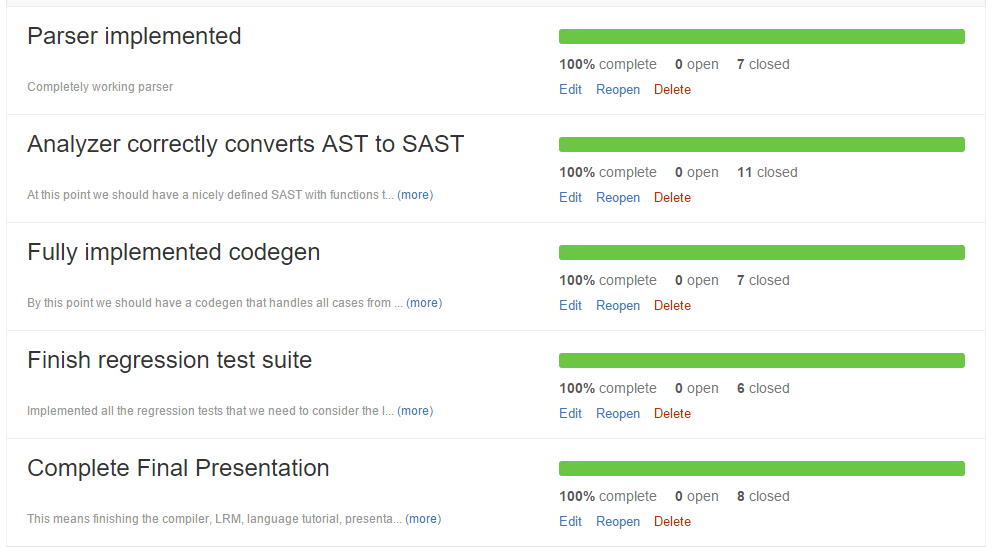
\includegraphics[width=4.5in]{Includes/milestones}
		\caption{Milestoning on Github.}
	\end{figure}
	
	\section{Specification Process}
	At the beginning of the semester we had originally intended our language to be a distributed software solution that would conveniently allow the developer to distribute tasks to various slave machines that had compiled the tasks to LLVM IR. After discussing this with professor Edwards we then decided to opt for an object oriented programming language that specifically compiled to LLVM IR. This way we as a team could learn more about making compilers and showing the power of LLVM. 
	
	Once we decided on the theme of Dice, we met to discuss the features we wanted most in our object oriented language. In our case we wanted arrays, inheritance, objects, and file IO to be some of the key highlights of our language. We then built up the scanner and parser to get a more solid idea as to what the language would look like, and by November 15th we had solidified our plans to implement the aforementioned features. 
	
	\section{Development Process}
	Implementation was very dependent on the course deadlines. We started with the scanner and parser specifically so the language reference manual was better defined. This was completed by October 26th. We then iterated on the analyzer and codegen until it was capable of producing hello world. This was completed on November 15th. The month afterwards was spent implementing inheritance and arrays until they were finally completed on December 18th. 
	
	\section{Testing Process}
	Throughout the development process we had numerous tests. The plan was to always have tests that were non-functional so a feature could then be implemented to get them working. If we encountered an error that we were unsure of how to fix, we added more error messages in our compiler until we could exactly pinpoint where the error was occurring. We also made a rule for our team to handle each and every exception that could occur as a custom error message to be printed out by the compiler. 
	
	\section{Team Responsibilities}
	Team responsibilities were divided up and evenly distributed amongst the four group members. While we could not adhere to a strict division of labor based on group member titles, every member contributed to the codebase. \\
	
	\begin{tabular}{|c|c|}
		\hline
		Team Member & Responsibility \\
		\hline
		David Watkins & Scanner, Parser, Analyzer, Codegen, Utils, LRM, Final Report, Latex, Code cleanup\\
		\hline
		Emily Chen & Inheritance in Analyzer, Expression types in Analyzer, LRM\\
		\hline
		Khaled Atef & Test Suite, Binary and unary expression evaluation in codegen\\
		\hline
		Phillip Schiffrin & Standard Library, Class map generation \\
		\hline
	\end{tabular}
	
	\section{Github Usernames}
	The following Github usernames correspond to the following group members:
	\begin{itemize}
		\item Emily Chen - six5532one, ec2805
		\item Khaled Atef - KhaledAtef
		\item David Watkins - DavidWatkins
		\item Phillip Schiffrin - nethacker11
	\end{itemize}
 
	\section{Project Log}
	To demonstrate our timeline we captured the number of git commits over time for our project. 
	
	\begin{figure}[!ht]
		\centering
		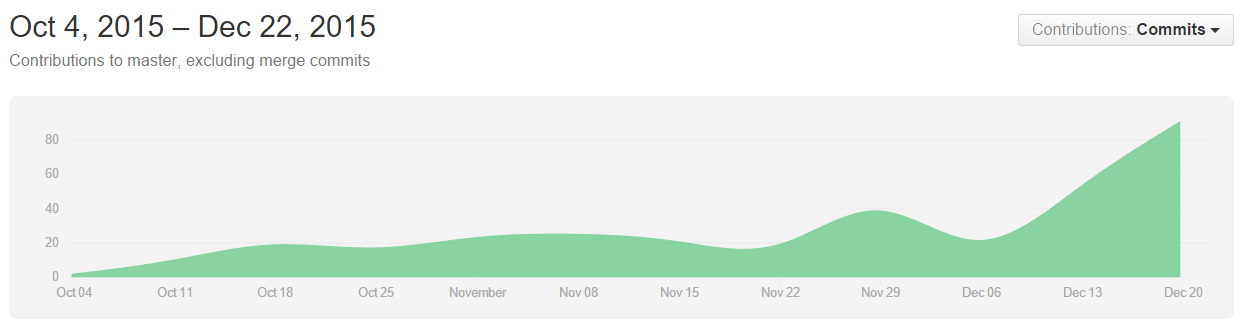
\includegraphics[width=5.5in]{Includes/timeline}
		\caption{Commit timeline on Github.}
	\end{figure}
	\pagebreak
	The timeline shows that we have been diligent at constantly working on the project since the beginning of the semester. All group members have contributed to this project. The following issues are a list of git issues that were cleared as part of our project, as well as the person who closed the issue. We did not have a rule for who closed an issue so sometimes the person who completed the issue may not have been the one to close it. 
	
	\begin{itemize}
		\item \#71 Should not be able to access variables outside of scope
		\item \#137 Awesome!
		\item \#134 Subclass assignment [by @six5532one, @DavidWatkins]
		\item \#133 string length tests
		\item \#132 fix delete test, no multiple arrays
		\item \#131 this should raise no exceptions
		\item \#130 Expected stderr: "exception Exceptions.LocalAssignTypeMismatch("B", "C")"
		\item \#129 passing in an inherited class for classes
		\item \#128 E-test-privateFieldsAccess.dice
		\item \#127 Create test for cyclical inheritance
		\item \#126 Add error message for assigning parameters
		\item \#125 test-gcd.dice Bug. You cannot assign values to parameters
		\item \#124 test-constructor1.dice is written incorrectly
		\item \#123 Maximum float is limited to 6 digits after the decimal
		\item \#122 char[][] args does not work in main
		\item \#121 Test max/min floats
		\item \#120 Test default constructor
		\item \#119 Test overloading std-lib functions
		\item \#118 Exit not working in runtime
		\item \#117 Test args
		\item \#116 assign ints to floats
		\item \#115 Integer toString generates string twice
		\item \#114 concat adds an extra character to the string
		\item \#113 Test exit
		\item \#111 Errors.log from script output isn't working properly
		\item \#110 add teststdlib .out
		\item \#109 Add Test returning objects
		\item \#108 add tests for empty blocks
		\item \#107 For inheritance of functions we should have an id to determine which function to call
		\item \#106 Includes should check with String\_lit not ID
		\item \#105 Odd invalid numbering of blocks bug
		\item \#104 Fix parameters on library functions
		\item \#103 Get Dice exec working so tests can run again.
		\item \#102 "Get the t-shirts made"
		\item \#101 Adapt codegen to changes in analyzer that add inherited fields to sprogram.classes
		\item \#100 Need to test includes
		\item \#99 add test for empty conditionals
		\item \#98 add empty for loop test
		\item \#97 Add nested comments
		\item \#96 test order of fdecl,fields,constructor in classses
		\item \#95 primitive type limit tests
		\item \#94 test constructors
		\item \#93 test private scope function
		\item \#92 Help needed: env.env\_class\_maps seems correct but exception is raised when I try to access an inherited field
		\item \#91 default constructors
		\item \#90 Need to add an environment variable to point to the includes
		\item \#89 Strings need to be initialized and accessed differently from normal arrays
		\item \#88 This should raise "UndefinedClass: H"
		\item \#87 Use of Delete
		\item \#86 add static scoping test
		\item \#85 Add applicative order test
		\item \#84 Add delete command to free memory
		\item \#82 Add exit call
		\item \#81 return statements in branches aren't recognized
		\item \#80 dice executable doesn't run without any args
		\item \#79 Kappa [by @DavidWatkins]
		\item \#78 Add tests for recursion
		\item \#77 Obj access [by @DavidWatkins]
		\item \#75 Test invalid functions
		\item \#74 Test multiple classes
		\item \#73 Parent cannot have fields of type of its children
		\item \#72 Cannot call return inside of a constructor
		\item \#135 check for overridden methods takes ret type into account [by @six5532one, @DavidWatkins]
		\item \#69 Casting rules questions
		\item \#68 Kappa [by @DavidWatkins]
		\item \#67 Floats print with extra trailing zeros. Kinda ugly.
		\item \#66 Emily [by @six5532one, @DavidWatkins]
		\item \#65 local decl (primitives): stderr should be "DuplicateLocal: myc"
		\item \#64 object creation: this should raise no exception
		\item \#63 object creation: this should raise no exceptions
		\item \#62 Compiler doesn't allow formal to be an object
		\item \#61 object creation: This should throw no exceptions
		\item \#60 Object creation: this should raise "ConstructorNotFound: Foo.constructor.int.bool.char.float"
		\item \#59 object decl without assignment expr: This should throw no exceptions
		\item \#58 This should throw exception "UndefinedClass: Baz"
		\item \#57 incorrect check for duplicate constructors
		\item \#56 Emily [by @six5532one, @DavidWatkins]
		\item \#55 Create arith tests that have signed values
		\item \#54 Parser issue with reading user-defined objects.
		\item \#53 Emily [by @six5532one]
		\item \#52 Decide whether to promote all ints to floats in binops
		\item \#51 Consecutive print statements don't work. Compiler only outputs first print statement.
		\item \#50 Epsilon [by @six5532one]
		\item \#49 Reorganize object accesses for functions
		\item \#46 Kreygasm [by @DavidWatkins]
		\item \#45 Add shakespeare and stephen number to tester
		\item \#44 Create symbol table for cdecls, fdecls, fields
		\item \#39 static analysis checks for variable access
		\item \#38 use `new` keyword for object and array instantiation
		\item \#37 support addition of chars and ints
		\item \#36 Update LRM: support addition of chars and ints
		\item \#35 Change parser array create type to type tag and not primitive
		\item \#34 Evaluate whether to add new as a keyword to object initialization
		\item \#33 Exceptions, try, catch?
		\item \#32 Implement basic primitive expressions for codegen
		\item \#31 Should we add continuous checking even when an illegal character/parser error occurs like java?
		\item \#30 Add annotation for source code position to AST
		\item \#29 We should evaluate whether we want to move variable declarations to stmts
		\item \#28 Do we need to add an additional layer of abstraction from SAST to Codegen?
		\item \#27 Complete pretty printing abstract syntax tree to Utils
		\item \#26 How does LLVM handle allocating on the heap
		\item \#24 Strings with escape characters are not being displayed properly
		\item \#23 Create OCamlDoc Documentation
		\item \#22 Should we switch the llvm package to ollvm?
		\item \#21 Add file operator functions to Codegen
		\item \#20 Write the File class
		\item \#19 Write the String class
		\item \#18 Write the Math class
		\item \#17 Add support for utilizing line number and character number in Analyzer
		\item \#16 Add class name and function name collission detection
		\item \#15 Add testing for arrays
		\item \#14 Evaluate the type of an expression in Analyzer.get\_expr\_type
		\item \#13 Add testing for extends
		\item \#12 Add mentioning of unary minus to LRM
		\item \#11 Remove '-' symbol from regex in floats and ints of LRM
		\item \#10 Convert AST.cdecl to SAST.cdecl
		\item \#9 Convert AST.expr to SAST.expr in Analyzer.convert\_expr
		\item \#8 Analyzer.process\_includes does not check absolute path
		\item \#7 Delta [by @DavidWatkins]
		\item \#6 Delta [by @DavidWatkins]
		\item \#5 Special chars (tabs/newlines/etc) aren't getting tokenized properly
		\item \#4 float limit
		\item \#3 David fix [by @DavidWatkins]
		\item \#2 Merge pull request \#1 from DavidWatkins/DavidFix [by @DavidWatkins]
		\item \#1 David fix [by @DavidWatkins]
	\end{itemize}
	\section{Git Commit History}
	Here are all of the commits as performed by the team. Everyone contributed to the project.
	\begin{minted}[linenos]{text}
commit 738b0558ddb9fe894a7611be0f1f9f590f38094a
Merge: 700e197 df6915a
Author: David Watkins <djrival7@gmail.com>
Date:   Tue Dec 22 20:45:33 2015 -0500

    Merge branch 'master' of https://github.com/DavidWatkins/DiceLanguage

commit 700e1979474d977ffb3496c7435f4f9dbace09e2
Author: David Watkins <djrival7@gmail.com>
Date:   Tue Dec 22 20:39:19 2015 -0500

    Added changes to standard library description

commit df6915a7d7a802e673daca3a6b364060b024035b
Merge: 8ac36b8 dbf27d2
Author: nethacker11 <philip.schiffrin@gmail.com>
Date:   Tue Dec 22 20:34:58 2015 -0500

    Merge branch 'master' of https://github.com/DavidWatkins/Dice

commit 8ac36b8a6d9714d1f096f8c8e990da9bd971afe7
Author: nethacker11 <philip.schiffrin@gmail.com>
Date:   Tue Dec 22 20:34:51 2015 -0500

    CFuncs.tex added

commit dbf27d2d940c93f0de61a210f98167faefeae014
Author: David Watkins <djrival7@gmail.com>
Date:   Tue Dec 22 20:28:22 2015 -0500

    Added grammar and small changes to lrm

commit 421588dcb8b30f42134c880143492e4822dbba2e
Author: nethacker11 <philip.schiffrin@gmail.com>
Date:   Tue Dec 22 20:23:33 2015 -0500

    added Builtin.tex

commit 0ec68907641d9be8a992b3dd7b023ec8e4f48afc
Merge: ef75162 ea3b98f
Author: David Watkins <djrival7@gmail.com>
Date:   Tue Dec 22 19:46:19 2015 -0500

    Merge branch 'master' of https://github.com/DavidWatkins/DiceLanguage

commit ef75162bd113e48a2ba794aa7ce002b613eeae3c
Author: David Watkins <djrival7@gmail.com>
Date:   Tue Dec 22 19:45:53 2015 -0500

    Added additional code for test plan in final report

commit ea3b98f6be0be4f8a66158b94d8391cd7b719948
Merge: 8524dfd 6378550
Author: nethacker11 <philip.schiffrin@gmail.com>
Date:   Tue Dec 22 19:45:41 2015 -0500

    Merge branch 'master' of https://github.com/DavidWatkins/Dice

commit 8524dfd397ddf421dcf7c7bd948649a825c355f5
Author: nethacker11 <philip.schiffrin@gmail.com>
Date:   Tue Dec 22 19:45:33 2015 -0500

    updated standard library in Library.tex

commit 63785501516be9117a65f4bc0908396b5496058c
Merge: 48d7e07 035c054
Author: David Watkins <djrival7@gmail.com>
Date:   Tue Dec 22 19:12:36 2015 -0500

    Merge branch 'master' of https://github.com/DavidWatkins/DiceLanguage

commit 48d7e0772b5cfe8e899efecb622041b198199497
Author: David Watkins <djrival7@gmail.com>
Date:   Tue Dec 22 19:12:14 2015 -0500

    Added additional stuff to proposal and tutorial

commit 035c054a00bf0ccc1b2b8d2dc1809f6fbab4dc08
Author: Khaled Atef <kaa2168@columbia.edu>
Date:   Tue Dec 22 19:11:12 2015 -0500

    Added Test Plan and Khal lessons learned to Final Report directory

commit 39a768eca63505299bfacc07eef0322753a4de64
Author: nethacker11 <philip.schiffrin@gmail.com>
Date:   Tue Dec 22 18:59:25 2015 -0500

    updated Syntax.tex for final report

commit 41e9106396bb0b2e693dd35bfd131151c7c1b641
Author: David Watkins <djw2146@columbia.edu>
Date:   Tue Dec 22 18:28:54 2015 -0500

    ADedd more stuf

commit c58d595f376df552bb65e1fdb33ec05a674eb8cd
Author: David Watkins <davidw@tkins.me>
Date:   Tue Dec 22 18:23:32 2015 -0500

    Added Demo_Animals to tex file

commit afa84191ecd40be39d14295c6c1f3fa25e7be6f6
Author: David Watkins <davidw@tkins.me>
Date:   Tue Dec 22 18:19:54 2015 -0500

    Fixed hello world demo breaking tests

commit 7e2a1b9e07040cb9929b5dc971a297c83b0a9fe1
Author: David Watkins <davidw@tkins.me>
Date:   Tue Dec 22 18:14:31 2015 -0500

    iejsiu

commit ab07735004b3f480677e269e65e9f009e9f10bdb
Author: David Watkins <davidw@tkins.me>
Date:   Tue Dec 22 18:12:52 2015 -0500

    ijij

commit b21f0885522047bf0a62afb4da5edb292958ade4
Author: David Watkins <davidw@tkins.me>
Date:   Tue Dec 22 18:11:09 2015 -0500

    Maybe this works?

commit 5dd98b2548b8718ebf8342ef3460bfa740a6ffad
Author: David Watkins <davidw@tkins.me>
Date:   Tue Dec 22 15:20:54 2015 -0500

    Fixed another bug

commit d6b49aae775f433bc4c733ef539f9d5b84605c6f
Author: David Watkins <djw2146@columbia.edu>
Date:   Tue Dec 22 15:19:31 2015 -0500

    updated code.texY

commit d92d49c30ebe2da66203d0eb28db41d78b0d9ec5
Author: David Watkins <davidw@tkins.me>
Date:   Tue Dec 22 15:17:11 2015 -0500

    Fixed tests

commit cfebb0d5104705df4e358b35879645c6f5190439
Author: David Watkins <davidw@tkins.me>
Date:   Tue Dec 22 15:09:13 2015 -0500

    Fixed section title on tests

commit b8e048f0a326c3fc4fccee0a99928aa0564f8233
Merge: e94920a 07ee0b6
Author: David Watkins <davidw@tkins.me>
Date:   Tue Dec 22 15:06:33 2015 -0500

    Merge branch 'master' of https://github.com/DavidWatkins/Dice

commit e94920ae5f16643a0f5ae85393d7cae7e8dc58f5
Author: David Watkins <davidw@tkins.me>
Date:   Tue Dec 22 15:06:16 2015 -0500

    Added code for adding tests to final report

commit 07ee0b6cc870f6a7c171d159a85f8c142807f6f7
Author: David Watkins <DavidWatkins@users.noreply.github.com>
Date:   Tue Dec 22 13:59:47 2015 -0500

    Update README.md

commit a16003fbdec97727c492c857335bc93478a50a70
Author: David Watkins <djw2146@columbia.edu>
Date:   Tue Dec 22 05:15:01 2015 -0500

    Added basis for final project report

commit f3e5fe83dae72565f2950c096c6ff0efecb1b567
Author: David Watkins <davidw@tkins.me>
Date:   Tue Dec 22 04:46:38 2015 -0500

    Need to fixed error tests

commit e16dc0448ac4444fe75f7fee46b10825fda2ba6d
Author: David Watkins <djrival7@gmail.com>
Date:   Mon Dec 21 20:14:33 2015 -0500

    Added presentation

commit 0bc2d56336f2bed25b1715a1b5c632a49147eea8
Author: Khaled Atef <kaa2168@columbia.edu>
Date:   Mon Dec 21 15:25:43 2015 -0500

    Logo modified

commit d39a5d9feb9ba50426b6caa3c32668ab57c410c5
Author: David Watkins <davidw@tkins.me>
Date:   Mon Dec 21 14:23:01 2015 -0500

    Finished demo code

commit c0ccf162f43b88ef2c732de15acd419250e5db5c
Author: David Watkins <davidw@tkins.me>
Date:   Mon Dec 21 14:21:42 2015 -0500

    Removed unecessary files

commit a03afb187f7b93c8c05874e1357975d3edf69fac
Author: David Watkins <davidw@tkins.me>
Date:   Mon Dec 21 13:55:16 2015 -0500

    Fixed the demo

commit eec6e6f7989d4022ac261cc453bb7646e84e0a69
Author: Khaled Atef <kaa2168@columbia.edu>
Date:   Mon Dec 21 07:31:49 2015 -0500

    input/output coordinated

commit ca6abe8eeda764edfa1c2abd2bce730619ee53c9
Author: Khaled Atef <kaa2168@columbia.edu>
Date:   Mon Dec 21 07:02:23 2015 -0500

    basics implemented for demo

commit 8d2eda8d25c81a0294b3cc52c285c76314600870
Author: Khaled Atef <kaa2168@columbia.edu>
Date:   Mon Dec 21 06:23:25 2015 -0500

    modified ascii art for demo

commit 0a3a0c3958e224b1883714e99bd317624dd5514b
Merge: 96d30dd 2437414
Author: Khaled Atef <kaa2168@columbia.edu>
Date:   Mon Dec 21 06:18:42 2015 -0500

    Merge branch 'master' of https://github.com/DavidWatkins/Dice

commit 96d30ddc28576c7013902f157a5435315967ddd1
Author: Khaled Atef <kaa2168@columbia.edu>
Date:   Mon Dec 21 06:18:36 2015 -0500

    file for demo

commit 24374142973e158c61ea3955ac8d963599a2b75d
Author: Khaled Atef <kaa2168@columbia.edu>
Date:   Mon Dec 21 05:57:03 2015 -0500

    Othello still broken after many compiler errors

commit b5fbea0a2101e0c18d6bc476f0e7dfc18539c356
Merge: bff1792 502eff9
Author: Emily Chen <emchennyc@gmail.com>
Date:   Mon Dec 21 02:39:56 2015 -0500

    Merge branch 'master' of https://github.com/DavidWatkins/Dice

commit bff17927857bd562451279c9109ba57f01469829
Author: Emily Chen <emchennyc@gmail.com>
Date:   Mon Dec 21 02:39:00 2015 -0500

    halfway through translating OthelloGame

commit 502eff9a39c369dcd131c4b36220018c0e16fbc4
Merge: 4da809d 79744e6
Author: nethacker11 <philip.schiffrin@gmail.com>
Date:   Mon Dec 21 02:35:23 2015 -0500

    Merge branch 'master' of https://github.com/DavidWatkins/Dice

commit 4da809d3964870b705e10f8126e77e80c152474f
Author: nethacker11 <philip.schiffrin@gmail.com>
Date:   Mon Dec 21 02:34:47 2015 -0500

    updated humanplayer, doesn't work

commit 79744e6e61a16d7e049323d5af621e6be2049bb6
Merge: 1086a20 76df32a
Author: Khaled Atef <kaa2168@columbia.edu>
Date:   Mon Dec 21 02:10:20 2015 -0500

    Merge branch 'master' of https://github.com/DavidWatkins/Dice

commit 1086a2003fcf4604b4b799b3c3e18cbb05901b48
Author: Khaled Atef <kaa2168@columbia.edu>
Date:   Mon Dec 21 02:10:11 2015 -0500

    First round of edits to parserScanner regex rules

commit 76df32ae8b70759eeddb134f57b8e3f6403e2e5f
Merge: 8a75b65 fb0a776
Author: Emily Chen <emchennyc@gmail.com>
Date:   Mon Dec 21 02:08:18 2015 -0500

    Merge branch 'master' of https://github.com/DavidWatkins/Dice

commit 8a75b65ddc464749d36e7998dcd243e8ef47b241
Author: Emily Chen <emchennyc@gmail.com>
Date:   Mon Dec 21 02:07:45 2015 -0500

    includes classes HumanPlayer, Player, LocationObj

commit fb0a7763290ca205303a36e595792cabc8bda14b
Author: nethacker11 <philip.schiffrin@gmail.com>
Date:   Mon Dec 21 02:04:24 2015 -0500

    updated demo files

commit a7e0a84173eee4c06f0413a7b8bde8c3a3ee1844
Author: nethacker11 <philip.schiffrin@gmail.com>
Date:   Mon Dec 21 01:10:57 2015 -0500

    updated demo stuff

commit c5882be1259eee843e06004c347cc1d047c79851
Merge: e91324a 15fe681
Author: nethacker11 <philip.schiffrin@gmail.com>
Date:   Sun Dec 20 23:38:05 2015 -0500

    Merge branch 'master' of https://github.com/DavidWatkins/Dice

commit e91324aef67a7876f967e35b4f4a6ca323af95f7
Author: nethacker11 <philip.schiffrin@gmail.com>
Date:   Sun Dec 20 23:35:45 2015 -0500

    added toInteger in stdlib

commit 15fe681f3b48135f96cfcf0c191bd6989b76fad9
Author: Khaled Atef <kaa2168@columbia.edu>
Date:   Sun Dec 20 22:19:03 2015 -0500

    125 tests working!

commit 9dc00916011d9c69d13ff247268e615c2b0ac122
Author: David Watkins <davidw@tkins.me>
Date:   Sun Dec 20 21:50:00 2015 -0500

    OthelloRunner Basic working

commit 9451871b5f68a79f41c4c463894b0cb6cf802b1f
Merge: e6007de bed598a
Author: Khaled Atef <kaa2168@columbia.edu>
Date:   Sun Dec 20 21:21:19 2015 -0500

    Merge branch 'master' of https://github.com/DavidWatkins/Dice

commit e6007de0f670b43d7ff183860c77b95e0d381b99
Author: Khaled Atef <kaa2168@columbia.edu>
Date:   Sun Dec 20 21:21:04 2015 -0500

    first draft Othello

commit bed598a8d60c21c69228029a024e7a5c3526c77d
Author: David Watkins <davidw@tkins.me>
Date:   Sun Dec 20 21:09:58 2015 -0500

    Got object access working

commit d82e1a593479bd9dd04454014feedfa7dab7f0b4
Author: Khaled Atef <kaa2168@columbia.edu>
Date:   Sun Dec 20 20:53:29 2015 -0500

    fileio test output works!

commit f000aa8d545bb8450340105b070501e9c242bcf1
Author: Khaled Atef <kaa2168@columbia.edu>
Date:   Sun Dec 20 20:50:32 2015 -0500

    removed delete test

commit 9a1f7cde27e9c688ec84ad76385e27ffd1e7dcb1
Merge: 4c82a21 41949c7
Author: David Watkins <davidw@tkins.me>
Date:   Sun Dec 20 20:45:44 2015 -0500

    Merge branch 'master' of https://github.com/DavidWatkins/Dice

commit 41949c76776af134beb6de2a473e3e869403a2d5
Author: Khaled Atef <kaa2168@columbia.edu>
Date:   Sun Dec 20 20:45:29 2015 -0500

    Modified output to match test

commit 4c82a21756ba8abf9aa149d16f9b949e4b3f80c4
Author: David Watkins <davidw@tkins.me>
Date:   Sun Dec 20 20:45:17 2015 -0500

    test-fileio now prints and writes itself

commit f86d9cb3250e36ac60bcdc42d65fce9d63bfda90
Merge: 39fea6b 0d28a10
Author: Khaled Atef <kaa2168@columbia.edu>
Date:   Sun Dec 20 20:40:33 2015 -0500

    Merge branch 'master' of https://github.com/DavidWatkins/Dice

commit 0d28a10d1ae9333877cdadd0f7eb7c99a587d561
Author: David Watkins <davidw@tkins.me>
Date:   Sun Dec 20 20:39:55 2015 -0500

    Fixed file io

commit 39fea6ba072e0eb973deadf72c28dc70140432c3
Author: Khaled Atef <kaa2168@columbia.edu>
Date:   Sun Dec 20 20:23:11 2015 -0500

    new tests

commit f989f8fcd03394dd759d65be5fa93406e7300fe8
Merge: ea1fc65 83d8ac3
Author: David Watkins <DavidWatkins@users.noreply.github.com>
Date:   Sun Dec 20 19:17:14 2015 -0500

    Merge pull request #135 from DavidWatkins/fix-overrides-check
    
    check for overridden methods takes ret type into account

commit ea1fc652a4bdde559280c96e38a01cd5ac165783
Merge: 0c7039c 3163d40
Author: David Watkins <DavidWatkins@users.noreply.github.com>
Date:   Sun Dec 20 19:16:39 2015 -0500

    Merge pull request #134 from DavidWatkins/subclass_assignment
    
    Subclass assignment

commit 0c7039c8d05f1a359ce8af67ed3fc0c581770539
Author: David Watkins <davidw@tkins.me>
Date:   Sun Dec 20 19:11:32 2015 -0500

    Fixed assignment of obj_access problem

commit 6aeaa4c8a0d3fe6852c80263c918334a0d22dc06
Author: David Watkins <davidw@tkins.me>
Date:   Sun Dec 20 18:51:03 2015 -0500

    Fixed stringClassReverse

commit 37ac35175eb27c39665b4bf77ee71d4a566bab4a
Author: David Watkins <davidw@tkins.me>
Date:   Sun Dec 20 18:26:16 2015 -0500

    Added array access on obj_access

commit 83d8ac3fa9a130f8667cd6cf82691e8738bc94d4
Author: Emily Chen <emchennyc@gmail.com>
Date:   Sun Dec 20 18:12:23 2015 -0500

    check for overridden methods takes ret type into account

commit 15d429843e5c9a584fa4914936df1ba3783b212f
Author: David Watkins <davidw@tkins.me>
Date:   Sun Dec 20 18:05:48 2015 -0500

    Fixed array create initialize

commit f2390b94a80cfff1c217b533cacf61d954bdfac3
Author: Khaled Atef <kaa2168@columbia.edu>
Date:   Sun Dec 20 17:49:22 2015 -0500

    tests...

commit 3163d400ace38ecdc60f41b643a27b9fa60dcd26
Author: Emily Chen <emchennyc@gmail.com>
Date:   Sun Dec 20 17:44:45 2015 -0500

    fixed formatting

commit ab4a07e9e55a5ce2db8f30782faa018b0762a53a
Author: David Watkins <davidw@tkins.me>
Date:   Sun Dec 20 17:39:11 2015 -0500

    Changed function naming collision schema

commit e91e642ad5fbfd8a64bea0b5e2295aaeb3ff4145
Author: Emily Chen <emchennyc@gmail.com>
Date:   Sun Dec 20 17:20:20 2015 -0500

    fixed subclass assignment not to raise exception with reg object creation

commit dba6456b40bf8fc2c032b34984c210c27352a4e2
Author: Emily Chen <emchennyc@gmail.com>
Date:   Sun Dec 20 16:48:52 2015 -0500

    checks subclass assignment

commit 0b512528037bec86727f7e721a08d636759ef845
Author: Khaled Atef <kaa2168@columbia.edu>
Date:   Sun Dec 20 16:45:20 2015 -0500

    more tests and fixes

commit dc3d893e18172bfa7fdb9733fb9990b22f26a3dc
Author: Khaled Atef <kaa2168@columbia.edu>
Date:   Sun Dec 20 16:12:12 2015 -0500

    cyclical inheritance test added

commit 00009886c90714b113bd2e9066df7c0314fe99be
Author: Khaled Atef <kaa2168@columbia.edu>
Date:   Sun Dec 20 15:52:35 2015 -0500

    inheritance object passed in arg test

commit 79585bfacf986d5b013396ecdea2c4ce1f078edd
Merge: ae4bcc4 b5d6640
Author: David Watkins <davidw@tkins.me>
Date:   Sun Dec 20 15:41:22 2015 -0500

    Merge branch 'master' of https://github.com/DavidWatkins/Dice

commit ae4bcc4ec6860484529e4431d96531ce245a3823
Author: David Watkins <davidw@tkins.me>
Date:   Sun Dec 20 15:40:50 2015 -0500

    Fixed way accessing inherited methods checker thing grammar english pls

commit b5d6640ecfe55fa20bc69d109be8ef38cb2df82a
Merge: 777db46 da9452f
Author: Khaled Atef <kaa2168@columbia.edu>
Date:   Sun Dec 20 15:30:29 2015 -0500

    Merge branch 'master' of https://github.com/DavidWatkins/Dice

commit 777db465f5de4f9ade562b56254806d86f884f88
Author: Khaled Atef <kaa2168@columbia.edu>
Date:   Sun Dec 20 15:30:18 2015 -0500

    more tests

commit b15dd23dd09a127b4b45eeef83bc8f284c86f3de
Author: Khaled Atef <kaa2168@columbia.edu>
Date:   Sun Dec 20 15:02:14 2015 -0500

    tests =0

commit da9452feecda712b24ae53419fc3858db4f7ffbb
Author: David Watkins <davidw@tkins.me>
Date:   Sun Dec 20 15:00:04 2015 -0500

    Fixed empty main problem

commit 7d23e2a16c131048d43fafa146b577ca5f18a8fb
Author: Khaled Atef <kaa2168@columbia.edu>
Date:   Sun Dec 20 14:52:01 2015 -0500

    fixed tests

commit dddd825bf32500fdd232c563c41b77a3e4426c44
Merge: 6b689f2 46d105a
Author: David Watkins <davidw@tkins.me>
Date:   Sun Dec 20 14:51:10 2015 -0500

    Merge branch 'master' of https://github.com/DavidWatkins/Dice

commit 6b689f2c8446921678637a0d876c4411bbaa360b
Author: David Watkins <davidw@tkins.me>
Date:   Sun Dec 20 14:50:51 2015 -0500

    Added casting to subtypes

commit 46d105aef7000673550854485f86d0359b0c8b00
Author: Khaled Atef <kaa2168@columbia.edu>
Date:   Sun Dec 20 14:39:13 2015 -0500

    more tests including cyclical includes

commit 81392df3b88074c974fe897d35ee65b3cfe026d4
Merge: 9ace750 9301a8c
Author: nethacker11 <philip.schiffrin@gmail.com>
Date:   Sun Dec 20 14:06:38 2015 -0500

    Merge branch 'master' of https://github.com/DavidWatkins/Dice

commit 9ace75050be810f9e0e460d47c409e972aaaa990
Author: nethacker11 <philip.schiffrin@gmail.com>
Date:   Sun Dec 20 14:06:23 2015 -0500

    added 2 tests

commit 9301a8c8bebadeb4cf67f4199b1084c9d25107b3
Merge: f9503b9 20c6b6c
Author: David Watkins <davidw@tkins.me>
Date:   Sun Dec 20 14:05:44 2015 -0500

    Merge branch 'master' of https://github.com/DavidWatkins/Dice

commit f9503b95b010f8c9516093fe1b9cac3f6e8a7f3c
Merge: df64b34 f17b85f
Author: David Watkins <davidw@tkins.me>
Date:   Sun Dec 20 14:05:29 2015 -0500

    Merge branch 'master' of https://github.com/DavidWatkins/Dice

commit 20c6b6c16425120bbe1da4d355178c054b384698
Author: Khaled Atef <kaa2168@columbia.edu>
Date:   Sun Dec 20 14:01:26 2015 -0500

    more tests passing

commit df64b347fd6e07abb2d4f0834da862231ff35cba
Author: David Watkins <davidw@tkins.me>
Date:   Sun Dec 20 13:49:00 2015 -0500

    Added some broken stuff

commit f17b85fedaf22ff07158c044185229a9d96f4f13
Author: nethacker11 <philip.schiffrin@gmail.com>
Date:   Sun Dec 20 13:46:57 2015 -0500

    added getchar()

commit 034b4a4e8a56c49e0de21385534708706f88f3af
Author: David Watkins <davidw@tkins.me>
Date:   Sun Dec 20 12:58:20 2015 -0500

    Functions now have working private scope

commit fef6f2a5139dd5dda3d0d00cb349898d584ac0da
Author: David Watkins <davidw@tkins.me>
Date:   Sun Dec 20 12:32:55 2015 -0500

    main args is now working

commit 47a6d182878aa980a372554b5eb7bd331cf60e7f
Author: David Watkins <davidw@tkins.me>
Date:   Sun Dec 20 11:26:54 2015 -0500

    Break and continue now work

commit a9be4f6c34ee4230620875dc92bd7f7489d66c5f
Author: David Watkins <davidw@tkins.me>
Date:   Sun Dec 20 10:01:28 2015 -0500

    Added code for checking if break or continue is valid

commit 795773d726798b0b7d698e35293f4ee76c2acdf4
Author: David Watkins <davidw@tkins.me>
Date:   Sun Dec 20 09:37:20 2015 -0500

    Added basic private checking, not working for inheritance

commit 2e1c681369eb3397f0de724572cdf413988efbaa
Author: David Watkins <davidw@tkins.me>
Date:   Sun Dec 20 08:54:08 2015 -0500

    Added casting at the beginning of overridden function

commit ca425b48bfa72b4f26d4f2be8bc92f69a4cb4fdf
Author: David Watkins <davidw@tkins.me>
Date:   Sun Dec 20 08:35:36 2015 -0500

    Added default constructor

commit 98e3f63c3121a86e40c4445ff4bdd7f7dff36893
Author: David Watkins <davidw@tkins.me>
Date:   Sun Dec 20 08:06:45 2015 -0500

    Virtual function resolution works

commit 145101c510c43fb8809e5fe2ccdd7de2e8ece722
Author: David Watkins <davidw@tkins.me>
Date:   Sun Dec 20 06:56:25 2015 -0500

    Added working vtbl

commit 21f7e5cc757e7f94f3d41e71c95590188119a15b
Author: David Watkins <davidw@tkins.me>
Date:   Sun Dec 20 05:26:16 2015 -0500

    Cleaned up use of types in SAST

commit 064f098e6ced5aa733a3beabf8edd3dda5173db3
Author: David Watkins <davidw@tkins.me>
Date:   Sun Dec 20 05:12:03 2015 -0500

    Added unused integer to all scalls

commit 9ee2d0ef828eff03f3acd0ed117610481d012135
Merge: 2042484 76746fd
Author: David Watkins <davidw@tkins.me>
Date:   Sun Dec 20 05:01:45 2015 -0500

    Merge branch 'master' of https://github.com/DavidWatkins/Dice

commit 2042484a2a9e8778eb1c4a86c00cb0ba8e5e0625
Author: David Watkins <davidw@tkins.me>
Date:   Sun Dec 20 05:01:23 2015 -0500

    Incorporated Emily's changes to Analyzer

commit 76746fdb001845cb72dd757f870fc985b4f2261a
Merge: fa8e2ee c0eedeb
Author: Khaled Atef <kaa2168@columbia.edu>
Date:   Sun Dec 20 03:20:05 2015 -0500

    Merge branch 'master' of https://github.com/DavidWatkins/Dice

commit fa8e2eea360f9b10e068fa1937317cafb003df12
Author: Khaled Atef <kaa2168@columbia.edu>
Date:   Sun Dec 20 03:19:53 2015 -0500

    more tests

commit c0eedebd7866f602cd79bf581ba5030f5a9a53e4
Author: David Watkins <davidw@tkins.me>
Date:   Sun Dec 20 03:15:15 2015 -0500

    Reformatted some code, fixed exit bug

commit 0a275a096762f01c506384a281c827a0689e8ab5
Author: Khaled Atef <kaa2168@columbia.edu>
Date:   Sun Dec 20 02:20:27 2015 -0500

    modified dice.ml to pass exceptions

commit d61f20801707ee4ac695135909823b3ee4b09073
Author: nethacker11 <philip.schiffrin@gmail.com>
Date:   Sun Dec 20 00:18:20 2015 -0500

    took out print stmt in stdlib

commit e1bc841aa24a9ef597e94232e04735c26c4276cd
Author: Khaled Atef <kaa2168@columbia.edu>
Date:   Sun Dec 20 00:06:16 2015 -0500

    More tests =)

commit 60a80460f04a4ffe25d7bbe319734bab7c8ebc82
Author: nethacker11 <philip.schiffrin@gmail.com>
Date:   Sat Dec 19 22:45:15 2015 -0500

    fixed concat in stdlib

commit 7ad7480ee90a8759271b0961507d7f084990a162
Author: Khaled Atef <kaa2168@columbia.edu>
Date:   Sat Dec 19 21:25:12 2015 -0500

    Added more tests and modified dice.ml to account for an exception to make the test script work

commit 1eeea68662d793173c0dd4587cd244eb379e3176
Merge: 3529056 50a7529
Author: David Watkins <davidw@tkins.me>
Date:   Sat Dec 19 17:20:15 2015 -0500

    Merge branch 'master' of https://github.com/DavidWatkins/Dice

commit 3529056aae15850c8e3ce00eb314e0393d5a1ff3
Author: David Watkins <davidw@tkins.me>
Date:   Sat Dec 19 17:19:43 2015 -0500

    Added changes to allow for exit

commit 50a7529746b3b7488fb038d75817983dcef56713
Merge: d2b04d3 3fd9fbf
Author: nethacker11 <philip.schiffrin@gmail.com>
Date:   Sat Dec 19 17:16:14 2015 -0500

    Merge branch 'master' of https://github.com/DavidWatkins/Dice

commit d2b04d339c239b0000ccfdde4b93ee3bfe13a878
Author: nethacker11 <philip.schiffrin@gmail.com>
Date:   Sat Dec 19 17:15:51 2015 -0500

    updated stdlib to include Integer and String has reverse()

commit 3fd9fbf47a382b0c8bc02e6f13e32c810f7f9807
Merge: 8ac9eed 14e1b19
Author: Khaled Atef <kaa2168@columbia.edu>
Date:   Sat Dec 19 16:46:38 2015 -0500

    Merge branch 'master' of https://github.com/DavidWatkins/Dice

commit 8ac9eed3f00065424b59350a074749246d411869
Author: Khaled Atef <kaa2168@columbia.edu>
Date:   Sat Dec 19 16:46:20 2015 -0500

    more tweaks to tests and script

commit 14e1b190bfb5972a1a0394a23be43f178eef971b
Author: David Watkins <davidw@tkins.me>
Date:   Sat Dec 19 16:31:22 2015 -0500

    Fixed codegen for char_lits to i8_t

commit d984aff231ee6eb90e5921994f5d6fd14e044a79
Author: nethacker11 <philip.schiffrin@gmail.com>
Date:   Sat Dec 19 16:19:40 2015 -0500

    added test cases and updated stdlib

commit ff79fff82264ba8743377b3515514df0a988d7fc
Merge: b336d0a 602dc41
Author: David Watkins <davidw@tkins.me>
Date:   Sat Dec 19 15:57:18 2015 -0500

    Merge branch 'master' of https://github.com/DavidWatkins/Dice

commit b336d0a6333387906a3a63d44541953e1c6a4616
Author: David Watkins <davidw@tkins.me>
Date:   Sat Dec 19 15:57:02 2015 -0500

    Added modulo

commit 602dc4179efe1a87778934fb87428ddd5ee72d90
Author: Khaled Atef <kaa2168@columbia.edu>
Date:   Sat Dec 19 15:55:55 2015 -0500

    corrected tester script to account for errors from exception tests

commit cedf61d44d4d5a1faf2424eb50cf983df9df22f3
Author: David Watkins <davidw@tkins.me>
Date:   Sat Dec 19 15:24:25 2015 -0500

    Fixed function element access

commit 664bef08cd785fcd8f862874acfce3ced40bc5d2
Author: nethacker11 <philip.schiffrin@gmail.com>
Date:   Sat Dec 19 15:16:10 2015 -0500

    added stdlib2 test and updated stdlib

commit f4a81c401d29969e5b341c99f2e68e003318bb2e
Merge: 285aa85 3b7465c
Author: nethacker11 <philip.schiffrin@gmail.com>
Date:   Sat Dec 19 15:14:14 2015 -0500

    Merge branch 'master' of https://github.com/DavidWatkins/Dice

commit 3b7465cf892745766ce5a4bf08e4fdbdb28468eb
Author: David Watkins <davidw@tkins.me>
Date:   Sat Dec 19 15:13:45 2015 -0500

    This time for sure!

commit 285aa8594fe6d3b1fea5e2983e5599cc19bec253
Merge: 3425edc d7ed17e
Author: nethacker11 <philip.schiffrin@gmail.com>
Date:   Sat Dec 19 15:10:53 2015 -0500

    Merge branch 'master' of https://github.com/DavidWatkins/Dice

commit d7ed17e991fa0322eac0a63f0b55c84d4e2c1115
Author: David Watkins <davidw@tkins.me>
Date:   Sat Dec 19 15:10:09 2015 -0500

    Fixed function param passing bug

commit 3425edceaa05209d8f57da67867dac753d0ea0bc
Merge: 41afbc1 97de937
Author: nethacker11 <philip.schiffrin@gmail.com>
Date:   Sat Dec 19 15:02:04 2015 -0500

    Merge branch 'master' of https://github.com/DavidWatkins/Dice

commit 41afbc17bf2426ee44dc27bd254b550edbd78245
Author: nethacker11 <philip.schiffrin@gmail.com>
Date:   Sat Dec 19 15:02:02 2015 -0500

    updated codegen for lseek

commit 97de93788f1701bcc7e334d8061fe58fca6a5d35
Author: David Watkins <davidw@tkins.me>
Date:   Sat Dec 19 15:01:22 2015 -0500

    Fixed codegen_call for lseek

commit 3d58076d10a7060f85dfb363ec5cbce759038257
Merge: 7413f9b 464fc4c
Author: nethacker11 <philip.schiffrin@gmail.com>
Date:   Sat Dec 19 14:57:34 2015 -0500

    Merge branch 'master' of https://github.com/DavidWatkins/Dice

commit 464fc4c5d6119034866a6118cce83e59a56b3520
Merge: 87f4d52 7a63abf
Author: David Watkins <davidw@tkins.me>
Date:   Sat Dec 19 14:55:19 2015 -0500

    Merge branch 'master' of https://github.com/DavidWatkins/Dice

commit 87f4d52f2e6d185d46bc29b8635c6f98d7eb7853
Author: David Watkins <davidw@tkins.me>
Date:   Sat Dec 19 14:55:02 2015 -0500

    Added lseek syntax to analyzer

commit 7413f9b0e14a20d00314556df6e6c4890fd243f3
Merge: 3c1c15b 7a63abf
Author: nethacker11 <philip.schiffrin@gmail.com>
Date:   Sat Dec 19 14:22:33 2015 -0500

    Merge branch 'master' of https://github.com/DavidWatkins/Dice

commit 7a63abffd7edafb87ecf82df2225e7ea2148eeb8
Merge: c482260 afae098
Author: Khaled Atef <kaa2168@columbia.edu>
Date:   Sat Dec 19 14:22:02 2015 -0500

    Merge branch 'master' of https://github.com/DavidWatkins/Dice

commit c48226078ee263889c6de75ff8d0f6f572a6a7ee
Author: Khaled Atef <kaa2168@columbia.edu>
Date:   Sat Dec 19 14:21:41 2015 -0500

    added stdlib string

commit 3c1c15b99113b0e570fa6625ba4a2a0ee1c917e5
Merge: 480dc4d afae098
Author: nethacker11 <philip.schiffrin@gmail.com>
Date:   Sat Dec 19 14:19:44 2015 -0500

    Merge branch 'master' of https://github.com/DavidWatkins/Dice

commit 480dc4d0c15a9c5cd5bccfb7c8d05aebb423b9e7
Author: nethacker11 <philip.schiffrin@gmail.com>
Date:   Sat Dec 19 14:18:18 2015 -0500

    changed stdlib

commit afae098e32e66e69b0349e9809ce6d237f451179
Merge: acbea61 404c6df
Author: David Watkins <davidw@tkins.me>
Date:   Sat Dec 19 14:17:52 2015 -0500

    Merge branch 'master' of https://github.com/DavidWatkins/Dice

commit acbea6113ddccfa59ce06c8288a4bfe81b134f6f
Author: David Watkins <davidw@tkins.me>
Date:   Sat Dec 19 14:17:31 2015 -0500

    Fixed right associativity of parser

commit 404c6df62cc80b61ceffed8cc666f9591757d5e0
Merge: 782ca3f 3e4e5e6
Author: Khaled Atef <kaa2168@columbia.edu>
Date:   Sat Dec 19 14:15:07 2015 -0500

    Merge branch 'master' of https://github.com/DavidWatkins/Dice

commit 17c1362a3d24b7edf544491948a259fb816524a4
Merge: c248f39 3e4e5e6
Author: nethacker11 <philip.schiffrin@gmail.com>
Date:   Sat Dec 19 14:15:07 2015 -0500

    Merge branch 'master' of https://github.com/DavidWatkins/Dice

commit c248f394794dc1a26b0052db05a4a2abffe5ba89
Author: nethacker11 <philip.schiffrin@gmail.com>
Date:   Sat Dec 19 14:15:05 2015 -0500

    updated stdlib

commit 782ca3fa5c903b0c87d7402724934c25a3cf3a30
Author: Khaled Atef <kaa2168@columbia.edu>
Date:   Sat Dec 19 14:14:49 2015 -0500

    modified tests

commit 3e4e5e6b27248dbe9de6af579040dbc991f2b5be
Author: David Watkins <davidw@tkins.me>
Date:   Sat Dec 19 14:13:16 2015 -0500

    Fixed array access for chars

commit cbcdff6c41b458da3355bf3aecb58a5d3549752e
Merge: 3ca5e39 0c9870c
Author: David Watkins <davidw@tkins.me>
Date:   Sat Dec 19 13:54:44 2015 -0500

    Merge branch 'master' of https://github.com/DavidWatkins/Dice

commit 3ca5e39a56c7a6c239d38e9c58eabd03304f1526
Author: David Watkins <davidw@tkins.me>
Date:   Sat Dec 19 13:54:14 2015 -0500

    Fixed array acces for strings

commit 0c9870c3948b1e193926f363ec551830d8aae9ae
Author: Khaled Atef <kaa2168@columbia.edu>
Date:   Sat Dec 19 13:54:04 2015 -0500

    added more tests

commit 91c9bc47dff55afd6269202ad1654145cf55b5da
Author: David Watkins <davidw@tkins.me>
Date:   Sat Dec 19 05:07:25 2015 -0500

    Fixed stdlib

commit c603715b9036aa50daa30a423ee6e0b30fd9e8ce
Author: David Watkins <davidw@tkins.me>
Date:   Sat Dec 19 04:08:52 2015 -0500

    While loops work

commit 27b53ff8e9131b2e686ed29755d54690936a2131
Author: David Watkins <davidw@tkins.me>
Date:   Sat Dec 19 04:02:09 2015 -0500

    Fixed bug with array length

commit 64b72feeb55e71b92c1fd7810e5ccb82ae736f41
Author: David Watkins <davidw@tkins.me>
Date:   Sat Dec 19 03:39:57 2015 -0500

    Fixed odd incorrect ordering bug

commit 170e4fd2e2285c0d7f106426651199a48c5b20e6
Author: David Watkins <davidw@tkins.me>
Date:   Sat Dec 19 03:34:00 2015 -0500

    Fixed includes bug, fixed char array assignment of int length

commit 7c8d274ea55d5118e70db8f3d11dd5cff42d36e4
Author: David Watkins <davidw@tkins.me>
Date:   Sat Dec 19 01:36:29 2015 -0500

    Migrated files and folders to appropriate place for new makefile schema

commit a1ae8ffbc1d1fe84c755abf98a44392680a63c20
Author: nethacker11 <philip.schiffrin@gmail.com>
Date:   Fri Dec 18 22:57:30 2015 -0500

    updated stdlib and analyzer and codegen for built in functions

commit 1a5244813f0c299c673096a48a09dad022133599
Author: David Watkins <davidw@tkins.me>
Date:   Fri Dec 18 20:01:52 2015 -0500

    Fixed \0, its now \000

commit a2d07124a44c96af5b158996c049fead07644dc5
Author: nethacker11 <philip.schiffrin@gmail.com>
Date:   Fri Dec 18 20:02:58 2015 -0500

    updated stdlib.dice

commit e9c8d476beb76ebd9a4f4d1a23f5cf722d741744
Author: David Watkins <davidw@tkins.me>
Date:   Fri Dec 18 19:47:00 2015 -0500

    backslash zero yo

commit d6be8f34690274401b8123cf491254274e8030b9
Author: David Watkins <davidw@tkins.me>
Date:   Fri Dec 18 19:33:09 2015 -0500

    works now?

commit 8ad670e00d5b7cf8020581861306cf89ab17b8a6
Merge: aec396d c6af1ee
Author: David Watkins <davidw@tkins.me>
Date:   Fri Dec 18 19:17:00 2015 -0500

    Merge branch 'master' of https://github.com/DavidWatkins/Dice

commit aec396db7c9a6714ce6e5de976596b42c1d03c8e
Author: David Watkins <davidw@tkins.me>
Date:   Fri Dec 18 19:16:41 2015 -0500

    Works *crosses fingers*

commit c6af1eecd3362b57591589d61493c14707c11479
Author: nethacker11 <philip.schiffrin@gmail.com>
Date:   Fri Dec 18 19:13:08 2015 -0500

    updated stdlib.dice

commit b0e033a148286f9de9c2cef0b37c799fb5ec36d0
Author: David Watkins <davidw@tkins.me>
Date:   Fri Dec 18 18:43:07 2015 -0500

    So uh, nested comments are a thing

commit 0e91f6aca66d2804747918f460114f356842befd
Author: Khaled Atef <kaa2168@columbia.edu>
Date:   Fri Dec 18 17:37:31 2015 -0500

    Exceptions folder created, need to add more tests here

commit 643197852baaf3fff864761ab7376bf32e6bacf0
Author: nethacker11 <philip.schiffrin@gmail.com>
Date:   Fri Dec 18 17:12:04 2015 -0500

    added stdlib.dice, passes analyzer but not tested

commit b9c354db5a56e4d8e9543a1c00147260283e5d51
Merge: 75cb0da 5ae669c
Author: Khaled Atef <kaa2168@columbia.edu>
Date:   Fri Dec 18 03:46:41 2015 -0500

    Merge branch 'master' of https://github.com/DavidWatkins/Dice

commit 75cb0daf1e69f062f9cb1e6c66079639ededd3e0
Author: Khaled Atef <kaa2168@columbia.edu>
Date:   Fri Dec 18 03:41:15 2015 -0500

    modified test script

commit 5ae669cf25734ab2bdfb6c989bfd933b98bdebb9
Author: David Watkins <davidw@tkins.me>
Date:   Thu Dec 17 19:26:41 2015 -0500

    Works?

commit 1cfe2ae2cf20eb203f45617097d9daa93abf3793
Author: nethacker11 <philip.schiffrin@gmail.com>
Date:   Thu Dec 17 19:24:59 2015 -0500

    added write function

commit 013f06fe8fcbf6d8db7dcf2cd32af311d47b7f2c
Merge: 4554586 b0dcfe9
Author: nethacker11 <philip.schiffrin@gmail.com>
Date:   Thu Dec 17 18:59:31 2015 -0500

    Merge branch 'master' of https://github.com/DavidWatkins/Dice

commit 4554586421327badd3daf2acb2c212fb98303a53
Author: nethacker11 <philip.schiffrin@gmail.com>
Date:   Thu Dec 17 18:59:29 2015 -0500

    added more build in function declarations

commit b0dcfe9708793c4946a123dbf45afea8c305027e
Author: David Watkins <davidw@tkins.me>
Date:   Thu Dec 17 18:58:19 2015 -0500

    Fixed shift/reduce, added linking of c functions

commit 9c7a140e1e036a70bb4af3159d21265a2799bcaf
Author: nethacker11 <philip.schiffrin@gmail.com>
Date:   Thu Dec 17 18:06:58 2015 -0500

    added c function declarations in codegen.ml under built in functions

commit d04c2b99e7c467914839a1b6429d7284d8c78725
Author: nethacker11 <philip.schiffrin@gmail.com>
Date:   Thu Dec 17 17:37:41 2015 -0500

    added folder for c library extensions for .bc files to be linked in dice.ml

commit d058e9c00fc86b609da0dce4a906b10718ca3430
Author: David Watkins <davidw@tkins.me>
Date:   Wed Dec 16 16:55:34 2015 -0500

    Added delete command to free memory

commit 9414ee274b553debcc02a052fff0fd34e46e14e8
Author: David Watkins <davidw@tkins.me>
Date:   Wed Dec 16 16:29:17 2015 -0500

    Added multi-dimensional c code

commit a08e96f67a96dd181abf6c67b769d371c326fa03
Author: David Watkins <davidw@tkins.me>
Date:   Wed Dec 16 16:28:52 2015 -0500

    Array length working, also added multi-dimensional c code

commit 59e4b9b012b92b799cdac22849c667130731163a
Author: David Watkins <davidw@tkins.me>
Date:   Wed Dec 16 01:41:37 2015 -0500

    Array primitives work

commit 3ab1e0ff494e1bdc57460aa3d930b5f15fe3c0a6
Author: David Watkins <davidw@tkins.me>
Date:   Tue Dec 15 23:45:42 2015 -0500

    Fixed single dimension arrays

commit f4ccfe7371bdd8c051db4735db872885a0578f42
Author: nethacker11 <philip.schiffrin@gmail.com>
Date:   Tue Dec 15 22:20:45 2015 -0500

    build_array_malloc in progress

commit 3e27ec7a42f5d91620f8c16390cf53a82f9e858f
Author: nethacker11 <philip.schiffrin@gmail.com>
Date:   Tue Dec 15 19:20:37 2015 -0500

    changing to single dimensional arrays, compiles but looks like arraycreate is not accessed again

commit 10e87f3b9c82258c06247f972144d63f582dbc4c
Author: David Watkins <davidw@tkins.me>
Date:   Tue Dec 15 18:44:34 2015 -0500

    Working status

commit c71bfa88710ef0a7c39f98fb4ece382a6dbb877c
Author: David Watkins <davidw@tkins.me>
Date:   Sat Dec 12 19:04:56 2015 -0500

    ArrayCreate doesn't work, added code for array deref

commit b9ed042660504b766617f397d21c8858756f4f95
Author: David Watkins <davidw@tkins.me>
Date:   Sat Dec 12 18:57:28 2015 -0500

    Added basic array methods

commit cdc675d5c824d42a7e82749a2472bb1da8726008
Author: David Watkins <davidw@tkins.me>
Date:   Fri Dec 11 15:28:10 2015 -0500

    Fixed bug where constructors weren't being checked by name

commit 8346a0009480db6799587fa8a1b3ab0178c5ea43
Author: David Watkins <DavidWatkins@users.noreply.github.com>
Date:   Thu Dec 10 18:18:39 2015 -0500

    Update README.md

commit b33b3a318fc92dbcdf434c72888f0c2399b3173f
Author: David Watkins <davidw@tkins.me>
Date:   Tue Dec 8 17:23:53 2015 -0500

    Added help printing to compiler with no arguments

commit ec57d8062f137244729246260d34a7cd47641525
Merge: ae65af0 bb7a89b
Author: David Watkins <DavidWatkins@users.noreply.github.com>
Date:   Sun Dec 6 17:21:44 2015 -0500

    Merge pull request #79 from DavidWatkins/Kappa
    
    Kappa

commit bb7a89b50cd1045cd8c0b711288d7bead3f8af20
Merge: ae65af0 43e4e3b
Author: David Watkins <davidw@tkins.me>
Date:   Sun Dec 6 17:21:21 2015 -0500

    Merge branch 'Kappa' of https://github.com/DavidWatkins/Dice into Kappa

commit ae65af04ea8c138768db9f1e25249d4c564d9882
Merge: 914b15a df7d695
Author: David Watkins <DavidWatkins@users.noreply.github.com>
Date:   Sat Dec 5 21:31:11 2015 -0500

    Merge pull request #77 from DavidWatkins/ObjAccess
    
    Obj access

commit df7d695d9f61cb7709ac5bd24422a23691d969dc
Author: David Watkins <davidw@tkins.me>
Date:   Sat Dec 5 21:29:47 2015 -0500

    Classes are now working, fixed tests to match up with new rules

commit 3547bd54ce8e66a8d984ecac37ef478f43d1d773
Author: David Watkins <davidw@tkins.me>
Date:   Fri Dec 4 15:39:07 2015 -0500

    Sigh

commit 914b15a3301e9de97ff5b9fcbf57f7731fbd90a0
Merge: bc5da4f b474701
Author: Khaled Atef <kaa2168@columbia.edu>
Date:   Fri Dec 4 01:27:57 2015 -0500

    Merge branch 'master' of https://github.com/DavidWatkins/Dice

commit bc5da4f925a2a6995b3d79cff92fff0f87f0384d
Author: Khaled Atef <kaa2168@columbia.edu>
Date:   Fri Dec 4 01:27:04 2015 -0500

    added else if tests

commit 43e4e3bf1d4a64e5fa71b3642a21250f37bb7334
Author: Khaled Atef <kaa2168@columbia.edu>
Date:   Fri Dec 4 01:14:26 2015 -0500

    unop working

commit 2fedba447dd85d89582b3aad84c0a470db87de7c
Author: David Watkins <davidw@tkins.me>
Date:   Wed Dec 2 17:14:26 2015 -0500

    Still WIP

commit a0c3cbf70c80847b0892ef61c9bf34c109ca1f49
Author: David Watkins <davidw@tkins.me>
Date:   Wed Dec 2 15:56:52 2015 -0500

    Added sample test script

commit a639719f7a7d885a4008be87ac94cbe5ec170695
Author: David Watkins <davidw@tkins.me>
Date:   Wed Dec 2 15:56:03 2015 -0500

    WIP

commit b47470171b10bbe3b8f7bcc9f7f0e52bf73a01e1
Author: David Watkins <DavidWatkins@users.noreply.github.com>
Date:   Wed Dec 2 07:33:33 2015 -0500

    Update README.md

commit 15e55374aea051650f8f627205dbcc8160544a75
Author: David Watkins <davidw@tkins.me>
Date:   Wed Dec 2 06:48:25 2015 -0500

    Function parameters are working

commit 0ff181573ba6a1fea1105ecc4b72f8fb269db965
Author: David Watkins <davidw@tkins.me>
Date:   Wed Dec 2 06:00:30 2015 -0500

    Added basic function calls to compiler

commit d99e2cc2f5b17ce3826ffe4aa0c6bc39e8297465
Author: Khaled Atef <kaa2168@columbia.edu>
Date:   Wed Dec 2 04:26:03 2015 -0500

    unop implemented, but not working. All tests are failing.

commit aaa1368f6872e5c20d669f38614fd431e3b21c65
Author: David Watkins <davidw@tkins.me>
Date:   Wed Dec 2 03:48:01 2015 -0500

    Added lazy evaluation and fixed error with function names

commit d0fa8223f546f315afc023d637f240af34329e36
Author: David Watkins <davidw@tkins.me>
Date:   Wed Dec 2 03:06:35 2015 -0500

    Changed wording in helper

commit 74059d062fdbbdc1679dac574052c05459751c08
Author: David Watkins <davidw@tkins.me>
Date:   Wed Dec 2 03:04:36 2015 -0500

    Added the ability to compile to a file

commit 2078c5fdb94b2cc6d265617c7d12d81e507c7e57
Author: Khaled Atef <kaa2168@columbia.edu>
Date:   Wed Dec 2 02:15:27 2015 -0500

    corrected test-bool4.dice

commit c0d5caee65fb50c2aa083309957bd1b20dba1c1c
Author: David Watkins <davidw@tkins.me>
Date:   Wed Dec 2 01:58:56 2015 -0500

    Float comparison expressions now evaluate properly

commit c6bb01085947ef3f51cbdc885238c3964039b708
Author: Khaled Atef <kaa2168@columbia.edu>
Date:   Wed Dec 2 01:29:37 2015 -0500

    fixed tests and added more for bools

commit 0d9c3a0dfe3b893c500f75090b5f04c89bb4401c
Merge: 63fdb09 a2300ae
Author: David Watkins <davidw@tkins.me>
Date:   Wed Dec 2 01:25:58 2015 -0500

    Merge branch 'master' of https://github.com/DavidWatkins/Dice

commit 63fdb093f7254bc4934fdde8b564b1d97463eada
Author: David Watkins <davidw@tkins.me>
Date:   Wed Dec 2 01:25:27 2015 -0500

    Added printing string representations of boolean values to codgen

commit a2300aedb2fe11c3fa612e1ae8f7d60537fb3019
Author: Khaled Atef <kaa2168@columbia.edu>
Date:   Wed Dec 2 00:36:29 2015 -0500

    Fixed syntax error

commit 861aee2ddb899d888a13e2a42e5a81c0a1528cd4
Merge: e7494e3 b0ab4a8
Author: Khaled Atef <kaa2168@columbia.edu>
Date:   Wed Dec 2 00:16:32 2015 -0500

    Merge branch 'master' of https://github.com/DavidWatkins/Dice

commit b0ab4a8e92319f72c3d1bb2376475b424cbf1887
Author: David Watkins <davidw@tkins.me>
Date:   Wed Dec 2 00:16:10 2015 -0500

    Reverted change to printing floats

commit e7494e3b6488dc49d28bb3bcad6e77f7ea42d265
Merge: d969ca2 21ac0fa
Author: Khaled Atef <kaa2168@columbia.edu>
Date:   Wed Dec 2 00:11:39 2015 -0500

    wMerge branch 'master' of https://github.com/DavidWatkins/Dice

commit d969ca2fc12093e18f946e893328b3cdb788ff43
Author: Khaled Atef <kaa2168@columbia.edu>
Date:   Wed Dec 2 00:11:08 2015 -0500

    nested if tests added with boolean tests of logical operators

commit 21ac0fa10db8c24347a0a56ed39cfc1b92e7ae19
Author: David Watkins <davidw@tkins.me>
Date:   Wed Dec 2 00:07:50 2015 -0500

    Fixed printing of floats

commit 4ca9ff15d8016c5fe78f81a23eb2b5bc19a443de
Author: David Watkins <davidw@tkins.me>
Date:   Tue Dec 1 23:52:18 2015 -0500

    Added exception for invalid integer operation in codegen

commit 9c25e446d76918a3b11be98a9d0aef72f2345e57
Merge: c45b5f8 72718b2
Author: David Watkins <DavidWatkins@users.noreply.github.com>
Date:   Tue Dec 1 23:50:17 2015 -0500

    Merge pull request #68 from DavidWatkins/Kappa
    
    Kappa

commit 72718b24c9c77818965340c2642b9746452517f9
Merge: 2031096 c45b5f8
Author: David Watkins <davidw@tkins.me>
Date:   Tue Dec 1 23:49:47 2015 -0500

    Merge branch 'master' into Kappa

commit 203109635a92704afcaf6ba8f7686e4bc56ee463
Author: Khaled Atef <kaa2168@columbia.edu>
Date:   Tue Dec 1 22:40:47 2015 -0500

    fixed unusued match warnings but matching AST type instead of llvalue. David determined that the Ocaml compiler can't tell the difference between i8_t and i32_t types.

commit c45b5f88281cfa8c5989fbc883bbe97230bac8c2
Merge: 3707602 7630cb1
Author: David Watkins <DavidWatkins@users.noreply.github.com>
Date:   Tue Dec 1 21:27:59 2015 -0500

    Merge pull request #66 from DavidWatkins/emily
    
    Emily

commit 7630cb139714b189697761faeb495d9a6d8055ad
Author: Emily Chen <emchennyc@gmail.com>
Date:   Tue Dec 1 21:26:16 2015 -0500

    raised wrong exception when trying to instantiate undefined class

commit 9d0040a4aa5506d46024e2c870dee099527cb6db
Author: Emily Chen <emchennyc@gmail.com>
Date:   Tue Dec 1 21:13:34 2015 -0500

    threw wrong exception for UndefinedClass case

commit 63765ae27d235ca0664cb329e72324475f80d6c0
Author: Emily Chen <emchennyc@gmail.com>
Date:   Tue Dec 1 20:26:28 2015 -0500

    object creation flags when actuals don't match any existing constructor

commit 1d3c59c8bf8ce3d1c621697025a9c529f0285a2c
Author: Emily Chen <emchennyc@gmail.com>
Date:   Tue Dec 1 17:26:18 2015 -0500

    types of actuals printed in same order as types of formals

commit 045fc2aa1cd78c1c93f58ce4c4412ccceada0b39
Author: Emily Chen <emchennyc@gmail.com>
Date:   Tue Dec 1 16:52:13 2015 -0500

    can print types of formals and actuals

commit 5e2ea6f7870c893d0e8fa6df422f3be55a240555
Author: Khaled Atef <kaa2168@columbia.edu>
Date:   Tue Dec 1 16:06:31 2015 -0500

    Test cases for arith negation added and build_global_stringptr modified for debugging

commit 4913954cb8166998c6aae53a2c1f733c06473890
Author: Khaled Atef <kaa2168@columbia.edu>
Date:   Tue Dec 1 08:43:55 2015 -0500

    added cast test (float+int)

commit b4f2afc359fb3ad8dcf1e658d428480c84c183a7
Author: Khaled Atef <kaa2168@columbia.edu>
Date:   Tue Dec 1 07:25:26 2015 -0500

    Compilesgit add codegen.ml !

commit 3ea9139620f9b937d7c6892cf1be2209cad34635
Author: Emily Chen <emchennyc@gmail.com>
Date:   Tue Dec 1 03:13:43 2015 -0500

    check_object_creation raises exception if instantiating unknown class

commit d98122c25680d734687c5e95d67832d620830d84
Author: Emily Chen <emchennyc@gmail.com>
Date:   Tue Dec 1 02:41:32 2015 -0500

    checks object decl to see if the class is available

commit 3bd51afa9cf5b2041543025837ed50d93ffe7d52
Author: Khaled Atef <kaa2168@columbia.edu>
Date:   Tue Dec 1 01:48:21 2015 -0500

    fought through several rounds of compilation errors.

commit 4494d69fc57cdac1a944a92ea7660f899a906a9f
Author: Khaled Atef <kaa2168@columbia.edu>
Date:   Tue Dec 1 01:22:02 2015 -0500

    Rough draft of handle_binop implemented. Still need to compile it, but pushing to access on VM. I hate OCaml

commit 37076028c622a12be9c222ca2331f265c99ac625
Author: David Watkins <DavidWatkins@users.noreply.github.com>
Date:   Mon Nov 30 23:49:19 2015 -0500

    Update README.md

commit 34586a39bbe449392a730dcbcf3e85dd2b70941c
Author: David Watkins <davidw@tkins.me>
Date:   Mon Nov 30 23:46:51 2015 -0500

    Merged Emily's changes to master

commit a2446010f6af0c06f465581a0b09bde85d4f1a3c
Author: David Watkins <davidw@tkins.me>
Date:   Mon Nov 30 23:41:58 2015 -0500

    Fixed pretty printer and loops

commit 9b8880077317b5dafd319becca52528d2fa8a393
Merge: 889c3b7 6f8b207
Author: David Watkins <DavidWatkins@users.noreply.github.com>
Date:   Mon Nov 30 23:35:44 2015 -0500

    Merge pull request #56 from DavidWatkins/emily
    
    Emily

commit 6f8b20749beb30748ed3912f631ad30cbfdf9ab0
Author: David Watkins <davidw@tkins.me>
Date:   Mon Nov 30 23:34:52 2015 -0500

    Added primitive variables

commit 1bfb88e3e588de2b2d097d9efa76cee25753129d
Author: Emily Chen <emchennyc@gmail.com>
Date:   Mon Nov 30 23:27:52 2015 -0500

    remove debugging statements

commit 0fe96a727e2fbd895fdc20e4bc3b4b423fcec17f
Merge: ef16286 889c3b7
Author: Emily Chen <emchennyc@gmail.com>
Date:   Mon Nov 30 22:41:57 2015 -0500

    Merge branch 'master' of https://github.com/DavidWatkins/Dice into emily

commit ef1628630066d0d7d20112a5def6a221fc38827c
Author: Emily Chen <emchennyc@gmail.com>
Date:   Mon Nov 30 22:41:07 2015 -0500

    converting local to slocal works for primitive types

commit 16491e2e0c6a513271acd0519f77b97818555344
Author: Emily Chen <emchennyc@gmail.com>
Date:   Mon Nov 30 22:01:09 2015 -0500

    local var decls are tracked even without assignment expr

commit 2adbb32da2aa5ccc60561594cb402d00b2e9c7bf
Author: Emily Chen <emchennyc@gmail.com>
Date:   Mon Nov 30 21:48:09 2015 -0500

    local var decl is added to env when statement includes nonempty expr

commit 889c3b715b50b63391a454a75a5d9d7dfbdd2657
Merge: 3064464 3d3154c
Author: David Watkins <davidw@tkins.me>
Date:   Mon Nov 30 19:49:10 2015 -0500

    Merge branch 'master' of https://github.com/DavidWatkins/Dice

commit 306446425bd29b931a6325b47b3da0cc3b84e04f
Author: David Watkins <davidw@tkins.me>
Date:   Mon Nov 30 19:48:49 2015 -0500

    Added pretty printing of sast and ast in JSON

commit 3d3154cea0c622561c7a63946e5e85ec8eb07e8d
Author: David Watkins <DavidWatkins@users.noreply.github.com>
Date:   Mon Nov 30 16:18:51 2015 -0500

    Update README.md

commit 64d255b692d1d3f156a210253bb4db2b1bd123ba
Author: Khaled Atef <kaa2168@columbia.edu>
Date:   Mon Nov 30 13:26:06 2015 -0500

    modified test script to perform automatic compilation of Dice Executable at the beginning of each session. Also, added -d flag to print any Dice Compiler messages to screen. Default is to print to log file

commit f4312c13faa500a2601e08b1fbd53568750df70b
Author: Khaled Atef <kaa2168@columbia.edu>
Date:   Mon Nov 30 12:14:07 2015 -0500

    corrected syntax error

commit b562f21c0f9e17dc946ddf2d1faa206346607e5d
Merge: 338553e db99c23
Author: David Watkins <davidw@tkins.me>
Date:   Mon Nov 30 08:10:05 2015 -0500

    Merge branch 'emily'

commit db99c2314ba0bdf2bba05501e971dd379e1a0bbc
Merge: 9f1d6c7 338553e
Author: David Watkins <davidw@tkins.me>
Date:   Mon Nov 30 08:09:54 2015 -0500

    Merge branch 'master' into emily

commit 338553e016ab991c9a5b278eb4e6fccb3e632121
Author: David Watkins <davidw@tkins.me>
Date:   Mon Nov 30 03:18:29 2015 -0500

    Added code for building for loops

commit ed35422de1e3530e82a4ecdb99a07c01774707cb
Merge: ac53ca3 7fe5c5c
Author: David Watkins <davidw@tkins.me>
Date:   Mon Nov 30 02:35:32 2015 -0500

    Merge branch 'master' of https://github.com/DavidWatkins/Dice

commit ac53ca3084d06312dabbe3058ab51694774c6bc3
Author: David Watkins <davidw@tkins.me>
Date:   Mon Nov 30 02:35:07 2015 -0500

    Fixed elseless if problem

commit 7fe5c5ca653e8a5973228953b681f431833a16bd
Merge: 9b5f7d1 50d5298
Author: Khaled Atef <kaa2168@columbia.edu>
Date:   Mon Nov 30 02:15:10 2015 -0500

    Merge branch 'master' of https://github.com/DavidWatkins/Dice

commit 9b5f7d18f8f895d4979b9a6bc32164262cb9bc31
Author: Khaled Atef <kaa2168@columbia.edu>
Date:   Mon Nov 30 02:14:35 2015 -0500

    basic inhertiance test added

commit 50d52984ad083eac3722a630cd027a0714537459
Merge: 75a41c3 1932754
Author: David Watkins <davidw@tkins.me>
Date:   Mon Nov 30 01:39:36 2015 -0500

    Merge branch 'master' of https://github.com/DavidWatkins/Dice

commit 75a41c3cf0da048bb6b76875f97d428cf84d8e41
Author: David Watkins <davidw@tkins.me>
Date:   Mon Nov 30 01:39:06 2015 -0500

    Ifs semi-implemented, multi-line programs work now

commit 9f1d6c75a4454794ac10e636bb6dd07291cbd642
Merge: a874f50 1932754
Author: Emily Chen <emchennyc@gmail.com>
Date:   Mon Nov 30 01:38:40 2015 -0500

    Merge branch 'master' of https://github.com/DavidWatkins/Dice into emily

commit a874f50a43d711086c8038dc92c06014bf11a39c
Author: Emily Chen <emchennyc@gmail.com>
Date:   Mon Nov 30 01:37:41 2015 -0500

    check_binop succeeds when only literal operands; doesn't handle IDs yet

commit 19327541aec867c8b3617ce7a55c2b8c30afc56a
Author: Khaled Atef <kaa2168@columbia.edu>
Date:   Mon Nov 30 01:35:32 2015 -0500

    array tests added for single and multidimensional arrays.

commit d1a88f6cc7a112e34869a03c36f0fbb8c95dea73
Author: Khaled Atef <kaa2168@columbia.edu>
Date:   Sun Nov 29 23:56:36 2015 -0500

    mroe tests

commit 01c53a3905d6dda85bd7d407ce1024c049401f3f
Merge: 0052631 96c9f21
Author: Emily Chen <emchennyc@gmail.com>
Date:   Sat Nov 28 16:48:45 2015 -0500

    Merge pull request #50 from DavidWatkins/epsilon
    
    Epsilon

commit 96c9f21a876921f9fe7b54c7c5520d2684926080
Merge: 0828f97 0052631
Author: Emily Chen <ec2805@columbia.edu>
Date:   Sat Nov 28 16:43:56 2015 -0500

    Merge branch 'master' of https://github.com/DavidWatkins/Dice into epsilon

commit 0828f97195361fcde1f315f76c0b9b40602fdfa6
Author: Emily Chen <ec2805@columbia.edu>
Date:   Sat Nov 28 16:43:40 2015 -0500

    current state of LRM, WIP

commit 00526316b382f1fcdbf7e20dd8116d76f3c0af49
Author: David Watkins <davidw@tkins.me>
Date:   Thu Nov 26 03:53:13 2015 -0500

    Added environments as return types for expressions and statements

commit 7bd0f08fd5735207d23ef0282f75571779c17032
Author: David Watkins <davidw@tkins.me>
Date:   Thu Nov 26 03:28:16 2015 -0500

    Added assignment type checking

commit 91f50320126a774977e963b002952cffcdaf8c0b
Author: David Watkins <davidw@tkins.me>
Date:   Thu Nov 26 03:18:53 2015 -0500

    Reorganized analyser unop

commit eb1e72d42ffccfa994b21db18c5ee7594b3086cb
Author: David Watkins <davidw@tkins.me>
Date:   Thu Nov 26 03:09:06 2015 -0500

    Print will now accept variable number of arguments and print integers

commit 2697f7d36eee3267d4d08acd72ee36218cfe885f
Author: David Watkins <davidw@tkins.me>
Date:   Thu Nov 26 02:43:40 2015 -0500

    Added reserved functions to analyzer

commit f016c356c05016b220b3503f7ef331c0cc6fe9e9
Author: David Watkins <davidw@tkins.me>
Date:   Wed Nov 25 23:14:40 2015 -0500

    Analyzer now uses SExpr instead of expr

commit 405feab53aeb98996d924e1d0c054b2c057893b8
Author: David Watkins <davidw@tkins.me>
Date:   Wed Nov 25 20:46:37 2015 -0500

    Added test ocaml code to produce llvm

commit fb92dc93387bc04a842ce20414642a8e0d6be079
Merge: a70917b d3bfd36
Author: Emily Chen <ec2805@columbia.edu>
Date:   Wed Nov 25 14:19:20 2015 -0500

    Merge branch 'master' of https://github.com/DavidWatkins/Dice into epsilon

commit d3bfd36c6a493a1c4b768bcc86049b5245975fdc
Author: David Watkins <davidw@tkins.me>
Date:   Mon Nov 23 03:55:35 2015 -0500

    Added a lot

commit 18c53d74b916b57cf79523da4bb5532408f0d623
Merge: e714714 c3635ab
Author: David Watkins <DavidWatkins@users.noreply.github.com>
Date:   Sat Nov 21 22:30:11 2015 -0500

    Merge pull request #46 from DavidWatkins/Kreygasm
    
    Kreygasm

commit c3635ab4859a46182ea3be101ffe08c80567da83
Author: nethacker11 <philip.schiffrin@gmail.com>
Date:   Sat Nov 21 22:28:57 2015 -0500

    duplicates checked in stringmaps

commit 347bb718b69bba5cedcf8d920e81fb46a9857602
Author: David Watkins <davidw@tkins.me>
Date:   Sat Nov 21 21:58:42 2015 -0500

    fubic

commit 796dad808edb739bb79e140ae8284affc416ba8e
Author: nethacker11 <philip.schiffrin@gmail.com>
Date:   Sat Nov 21 20:30:52 2015 -0500

    analyzer broken

commit 83453a96dc22e2b0cb3c0b5fadda6c38cd34f84d
Author: nethacker11 <philip.schiffrin@gmail.com>
Date:   Fri Nov 20 15:34:00 2015 -0500

    updated analyzer for global table

commit a70917bebd8b122fc1456a0de6d647f27e124378
Author: Emily Chen <ec2805@columbia.edu>
Date:   Tue Nov 17 05:39:53 2015 -0500

    specify wraparound behavior for char overflow during addition operation

commit 5ef7d4040ae2a3f384dc8e49108df9f911da54e8
Author: Emily Chen <ec2805@columbia.edu>
Date:   Tue Nov 17 05:32:45 2015 -0500

    fixed typos in Type section

commit 519ecd38eb0ff36345e404500a58799ab6e6f22e
Author: Emily Chen <ec2805@columbia.edu>
Date:   Tue Nov 17 05:32:15 2015 -0500

    fixed typos in Type section

commit 1dbea9cdd7ce99e8afb045d825c10cf7b61da1e6
Author: Emily Chen <ec2805@columbia.edu>
Date:   Tue Nov 17 05:28:27 2015 -0500

    lrm pdf

commit 218cdd226af54fc7a12aa54174686808b9c0c080
Author: Emily Chen <ec2805@columbia.edu>
Date:   Tue Nov 17 05:27:01 2015 -0500

    expressions emulate K&R reference

commit a23065b93cfa8ea563b2e5cafe47e4001364329f
Author: Emily Chen <ec2805@columbia.edu>
Date:   Tue Nov 17 04:14:47 2015 -0500

    remove examples from Types section

commit e71471403e598ff74fff7e1c18b6c26f84db7c4e
Author: Emily Chen <ec2805@columbia.edu>
Date:   Tue Nov 17 01:26:58 2015 -0500

    update regex for int, float

commit 01369938d06a83b7a411e97ea7f3105355ecb1c7
Author: David Watkins <davidw@tkins.me>
Date:   Mon Nov 16 21:09:30 2015 -0500

    Added new keyword, fixed pretty printing, allowed varied variable declaration

commit 90ac3e878efdb7d8471a49ac07b2717d568394ec
Author: David Watkins <davidw@tkins.me>
Date:   Mon Nov 16 05:00:47 2015 -0500

    Hello world demo code

commit 4a37b8b8e8fe6d695354db10b78f4273584ece35
Author: David Watkins <davidw@tkins.me>
Date:   Mon Nov 16 04:55:33 2015 -0500

    Added escape characters to string literals

commit cc898068bdd320886cbf6d6d950edc00a5cb8afe
Merge: be88ee9 d8ed6e5
Author: David Watkins <DavidWatkins@users.noreply.github.com>
Date:   Sun Nov 15 15:24:08 2015 -0500

    Merge pull request #7 from DavidWatkins/Delta
    
    Delta

commit be88ee9635bd7a60d134eac92cd8516dc08ccd06
Author: David Watkins <davidw@tkins.me>
Date:   Sun Nov 15 03:00:33 2015 -0500

    Removed bindings.c

commit b35203029ea05992df4d7356c556d8250379ec3e
Merge: 1a79286 bdfc46f
Author: David Watkins <davidw@tkins.me>
Date:   Sun Nov 15 02:55:59 2015 -0500

    Merge branch 'Delta' of https://github.com/DavidWatkins/Dice into HEAD

commit d8ed6e5ac77c66a1e28e43a91d1c7c90d10d096c
Merge: 819c652 bdfc46f
Author: David Watkins <davidw@tkins.me>
Date:   Sun Nov 15 02:49:47 2015 -0500

    Merge branch 'Delta' of https://github.com/DavidWatkins/Dice into Delta

commit bdfc46f92ab376ea29d6c672efa1c95cdc547f78
Author: Khaled Atef <kaa2168@columbia.edu>
Date:   Sun Nov 15 02:49:23 2015 -0500

    fixed cleaning up of temp files

commit 819c652f8af6058175b61339d75612f798b7f446
Author: David Watkins <davidw@tkins.me>
Date:   Sun Nov 15 02:43:59 2015 -0500

    Added unary minus

commit b79952cc5f486e080c31a7ae00b8977fa6812aa2
Author: David Watkins <davidw@tkins.me>
Date:   Sun Nov 15 02:37:18 2015 -0500

    Removed - from int and float literals

commit b7e306b4eb8dbb8859a79a7242064713f923605d
Author: David Watkins <davidw@tkins.me>
Date:   Sun Nov 15 02:29:54 2015 -0500

    Fixed rule with return

commit 30877b0821d29c59f8e86dbe8a0d4437d63dc6bc
Author: Khaled Atef <kaa2168@columbia.edu>
Date:   Sun Nov 15 02:21:01 2015 -0500

    tester corrected to work with lli

commit f037b3b5dc89409d59d55b5be4ed2a816b317be6
Merge: e843f0e ae1d756
Author: Khaled Atef <kaa2168@columbia.edu>
Date:   Sun Nov 15 02:19:51 2015 -0500

    Merge branch 'Delta' of https://github.com/DavidWatkins/Dice into Delta

commit e843f0ef31580d6846586a8ca49c2840222276c9
Author: Khaled Atef <kaa2168@columbia.edu>
Date:   Sun Nov 15 02:19:34 2015 -0500

    Corrected syntax errors in test case code

commit ae1d7560e16dd7eecdbc34a291d8f4e41a97eeeb
Author: David Watkins <DavidWatkins@users.noreply.github.com>
Date:   Sun Nov 15 02:10:16 2015 -0500

    Update README.md

commit 026fd5026bf957515f9b0902aa2d278b48197fe0
Author: David Watkins <DavidWatkins@users.noreply.github.com>
Date:   Sun Nov 15 01:55:44 2015 -0500

    Update README.md

commit 5ca0b69612e326f2523c5c7542f1ae5ea02d6f24
Author: David Watkins <davidw@tkins.me>
Date:   Sat Nov 14 20:14:41 2015 -0500

    Small edit to readme

commit 1c2547eef86a517507a6cbec1655f38df7875290
Author: David Watkins <davidw@tkins.me>
Date:   Sat Nov 14 20:12:53 2015 -0500

    Small changes

commit 54d7539d119aa459278dca7b3bcb68c248054948
Author: David Watkins <davidw@tkins.me>
Date:   Sat Nov 14 20:09:16 2015 -0500

    Added to README

commit d88306a8e86159b467a5da701bd315ce8e713d5a
Author: David Watkins <davidw@tkins.me>
Date:   Sat Nov 14 19:57:11 2015 -0500

    Compiler works, run build.sh

commit 32d87fa0fd8a81778ddd2d61936d64f5ef6aebc6
Author: Khaled Atef <kaa2168@columbia.edu>
Date:   Sat Nov 14 17:40:47 2015 -0500

    modified test script to use lli

commit 0db46dad8c7f8f97385be5602b4340efb7485c44
Merge: 8aa9ed2 2287265
Author: David Watkins <davidw@tkins.me>
Date:   Sat Nov 14 16:38:18 2015 -0500

    Merge branch 'Delta' of https://github.com/DavidWatkins/Dice into Delta

commit 8aa9ed21512f946604e9824e72d0f32f48460cb9
Author: David Watkins <davidw@tkins.me>
Date:   Sat Nov 14 16:37:59 2015 -0500

    Works!!!!!!

commit 228726581d0b46dd87aeeacfe2fc66b276ecd434
Merge: 01e738d 65f6ba6
Author: Khaled Atef <kaa2168@columbia.edu>
Date:   Sat Nov 14 16:19:25 2015 -0500

    Merge branch 'Delta' of https://github.com/DavidWatkins/Dice into Delta

commit 01e738dae2e637fd7a2265aa16bc3135172b24e2
Author: Khaled Atef <kaa2168@columbia.edu>
Date:   Sat Nov 14 16:11:58 2015 -0500

    testing script and basic test cases

commit 65f6ba6989f389b3db5b95cb4f0eaf0438f10157
Author: David <davidw@tkins.me>
Date:   Sat Nov 14 13:41:36 2015 -0500

    Made changes yo

commit 7dbe37512674db6a5f911bcc336878c45c5c1aca
Author: David <davidw@tkins.me>
Date:   Sat Nov 14 03:38:45 2015 -0500

    I give up for now

commit 04c4053bf43276ac073c4141ce1d2f79ddbc3452
Author: David <davidw@tkins.me>
Date:   Sat Nov 14 03:31:54 2015 -0500

    iWhatever

commit 1bfde45790ff5c37a06fed8a732d95343d6b09fe
Author: David Watkins <djw2146@columbia.edu>
Date:   Fri Nov 13 23:51:52 2015 -0500

    Again WIP

commit 6bc13cfadb5458a77b2d521390683981502d3cd1
Author: David Watkins <djw2146@columbia.edu>
Date:   Fri Nov 13 16:25:05 2015 -0500

    Added new way to make, figuring out layout for code based on tutorial

commit 1a79286feb4a6b21d8ded437dda312143a485f9b
Author: David Watkins <davidw@tkins.me>
Date:   Thu Nov 12 20:37:37 2015 -0400

    Wrong rule for utils

commit 550cd68be9b44ca6b4bb57dd3ca6539ae4ee04ca
Author: David Watkins <djrival7@gmail.com>
Date:   Wed Nov 11 15:44:05 2015 -0500

    Created base code for compiler and improved processinclude

commit e37f596018482de09bad4e87b85a9b346c33b374
Author: David Watkins <djw2146@columbia.edu>
Date:   Wed Nov 11 02:27:24 2015 -0500

    Added more descriptive error messages to dice files with incorrect syntax

commit 2c93957d1cf2401c8eae282123bcaa397290c194
Author: David Watkins <djw2146@columbia.edu>
Date:   Wed Nov 11 01:14:35 2015 -0500

    Changed primitive arrays to support inclusion of expressions and fixed
    escaped char literals

commit bfe58d3de921dd7428b6fb18d2ba2240336a0164
Merge: 13e70b1 77193cc
Author: Khaled Atef <kaa2168@columbia.edu>
Date:   Mon Nov 9 02:28:11 2015 -0500

    Merge branch 'master' of https://github.com/DavidWatkins/Dice

commit 13e70b1a603b87eb5c59dd96a7908a68e2b4286e
Author: Khaled Atef <kaa2168@columbia.edu>
Date:   Mon Nov 9 02:27:48 2015 -0500

    testing script implemented for Scanner tokenizer with some basic test cases. More to follow soon

commit 77193cc351212bbe8fd9ff02c73f71c2a958cf91
Author: Emily Chen <ec2805@columbia.edu>
Date:   Mon Nov 9 05:16:18 2015 +0000

    updated roles, re-rendered LRM pdf

commit 833154914d227be8b3d75ff2266cb5b1d016f185
Author: Emily Chen <ec2805@columbia.edu>
Date:   Mon Nov 9 05:13:39 2015 +0000

    updated roles

commit 48b5419853a7dad44ae3ef590ddb48f9f0fc40fb
Author: Emily Chen <ec2805@columbia.edu>
Date:   Mon Nov 9 05:08:07 2015 +0000

    updated LRM pdf

commit 62673cf7dcffe60a07ba5711e4df02c9d4542589
Author: Emily Chen <ec2805@columbia.edu>
Date:   Sun Nov 8 02:53:38 2015 +0000

    add description for logical operators and member access operator

commit 650993c85b05f1415aa1fedf4f995358d5e94f6b
Author: Emily Chen <ec2805@columbia.edu>
Date:   Sun Nov 8 02:24:12 2015 +0000

    add example of inheritance using "extends" kw

commit eb8488828a35dfe92828ff403eb3fa60b734eaf2
Author: Emily Chen <ec2805@columbia.edu>
Date:   Sun Nov 8 02:05:59 2015 +0000

    updated examples so they don't declare and initialize in same statement

commit ac91d9956899f8a7246bef381942afcf505f95b6
Author: Emily Chen <ec2805@columbia.edu>
Date:   Sun Nov 8 01:06:22 2015 +0000

    no class name collisions within module or between modules

commit 662d69a4aa9be43b54f85db25ec23ced249629b6
Author: Emily Chen <ec2805@columbia.edu>
Date:   Sun Nov 8 00:49:20 2015 +0000

    change .di to .dice; specify that recursive includes are not supported

commit 61afc126141b1ceaa5618ca4af55e1b6229a9f2f
Author: Emily Chen <ec2805@columbia.edu>
Date:   Sun Nov 8 00:39:14 2015 +0000

    describe Include statement

commit 9d04c148421a6793a71f17543fba74b0179b5a9e
Author: Emily Chen <ec2805@columbia.edu>
Date:   Sat Nov 7 23:59:35 2015 +0000

    updated array declaration, initialization, access in LRM

commit c73e469da24918a33fbc32fadf46eef0bb34a83d
Merge: 51f4c2e 18a9ca2
Author: David Watkins <djrival7@gmail.com>
Date:   Sat Nov 7 13:55:09 2015 -0500

    Merge branch 'master' of https://github.com/DavidWatkins/DiceLanguage

commit 51f4c2e5e49ea49f1b9d7fdc84b116f79da7ef74
Author: David Watkins <djrival7@gmail.com>
Date:   Sat Nov 7 12:16:59 2015 -0500

    Added nested primitive arrays to parser

commit 18a9ca288d017dffec5eb5240f6ed4e6551f4484
Author: Emily Chen <ec2805@columbia.edu>
Date:   Fri Nov 6 23:24:59 2015 +0000

     updated operator precedence in parser

commit 5a8cef865cec749060472a2da08f68e5f66ab603
Merge: 8a3a33b 233b9ae
Author: David Watkins <DavidWatkins@users.noreply.github.com>
Date:   Thu Nov 5 01:55:34 2015 -0500

    Merge pull request #3 from DavidWatkins/DavidFix
    
    David fix

commit 233b9ae4d2ad329217da5f89a02208e65f0f1056
Merge: 2339f25 8a3a33b
Author: David Watkins <DavidWatkins@users.noreply.github.com>
Date:   Thu Nov 5 01:51:37 2015 -0500

    Merge pull request #2 from DavidWatkins/master
    
    Merge pull request #1 from DavidWatkins/DavidFix

commit 2339f25231f1ee437ed6703545d6c7b010ec99a7
Author: David Watkins <djw2146@columbia.edu>
Date:   Thu Nov 5 01:47:31 2015 -0500

    Added AST printing method by using menhir inside ocaml

commit 8a3a33b299306b2322b4c87df2c42f559bb0f612
Merge: 9507d54 d095d57
Author: David Watkins <DavidWatkins@users.noreply.github.com>
Date:   Thu Nov 5 00:57:10 2015 -0500

    Merge pull request #1 from DavidWatkins/DavidFix
    
    David fix

commit d095d57af5fb83805fcbd5d70ff133facad7f64a
Author: David Watkins <djw2146@columbia.edu>
Date:   Thu Nov 5 00:37:34 2015 -0500

    Pretty printer bug fixed, tokenizer now prints line numbers

commit 7c800f61455e0a09d421afb4d384e1d0a07f5283
Author: David Watkins <djw2146@columbia.edu>
Date:   Wed Nov 4 22:12:26 2015 -0500

    Made changes to front end, pretty print and tokenizer work

commit b2a0bbd31c3484a2a914a1fb01cd8e05ecbc074f
Author: David Watkins <djw2146@columbia.edu>
Date:   Wed Nov 4 20:41:00 2015 -0500

    Fixed makefile?

commit 14f5ace95044a80e3d8d2a49e5e6a645f704a6ae
Author: David Watkins <djw2146@columbia.edu>
Date:   Wed Nov 4 20:35:55 2015 -0500

    This is just a test run of additional useful files, needs to be compiled
    on a unix system

commit a87e9b9a3706cb33fb79f260391b786bf53c6a40
Author: David Watkins <djrival7@gmail.com>
Date:   Wed Nov 4 15:57:22 2015 -0500

    Fixed parser with class keyword, removed array keyword

commit 41825d291a910847c3aa0d5d67f5c60f3698fcef
Author: David Watkins <djrival7@gmail.com>
Date:   Wed Nov 4 15:50:46 2015 -0500

    Revert "Fixed operator precedence"
    
    This reverts commit d132fdb8d21ba69a8d9d1c71c0ab71af5231eac0.

commit d132fdb8d21ba69a8d9d1c71c0ab71af5231eac0
Author: David Watkins <djrival7@gmail.com>
Date:   Wed Nov 4 15:24:56 2015 -0500

    Fixed operator precedence

commit 0726d908374df6c447d82290e06a83b84d0fdd0a
Author: David Watkins <djrival7@gmail.com>
Date:   Wed Nov 4 15:23:35 2015 -0500

    Fixed backet_args to refer to general expr list

commit ffec7d32cba2126885009518d79f072feea88628
Author: David Watkins <djrival7@gmail.com>
Date:   Wed Nov 4 15:21:37 2015 -0500

    Added datatypes to primitive arrays

commit 096f5a8bd45b44f23a42abaf837ad1f55597bce3
Author: David Watkins <djrival7@gmail.com>
Date:   Wed Nov 4 15:18:01 2015 -0500

    Fixed bug, apparently no issues wot

commit f30730a1cd041a3df6010c1ee62a59b17842e68f
Author: David Watkins <djw2146@columbia.edu>
Date:   Wed Nov 4 14:43:20 2015 -0500

    Fixed Menhir errors

commit 89a3de8e2e78735910eb385a3b51f4795e115c62
Author: David Watkins <djrival7@gmail.com>
Date:   Wed Nov 4 13:38:03 2015 -0500

    Removed extraneous files

commit c6d4db34bcca5aa6cc86a4e6f670a858c2f0b6bc
Author: David Watkins <djrival7@gmail.com>
Date:   Wed Nov 4 13:36:38 2015 -0500

    Cleaned up git directory

commit 4d157027e77211c94f295f34cef0d03a19c7f102
Author: David Watkins <djrival7@gmail.com>
Date:   Wed Nov 4 13:20:24 2015 -0500

    Found a more elegant solution to array problem

commit d7f28aa1dad4d1e788ab7b2aaab962372dfe1e71
Author: David Watkins <djrival7@gmail.com>
Date:   Wed Nov 4 00:06:05 2015 -0500

    No shift reduce but not ideal

commit d29a030e18489e489f0f8941cfbc70cc85c81a03
Author: David Watkins <djrival7@gmail.com>
Date:   Tue Nov 3 23:45:34 2015 -0500

    Super close, just ambiguity surroundign array access

commit 5473e62f147ec34eaccd4289930c4b2144d7c968
Author: David Watkins <djrival7@gmail.com>
Date:   Tue Nov 3 18:04:37 2015 -0500

    More stuff

commit dc6ad10dc89c389534ec225082c64da35a512268
Author: David Watkins <djrival7@gmail.com>
Date:   Tue Nov 3 14:10:00 2015 -0500

    Shift/Reduce down to 2, fixed layout of cdecl and cbody

commit 9507d5426cd130cc927941a4620383040c895717
Author: Khaled Atef <kaa2168@columbia.edu>
Date:   Mon Nov 2 13:07:36 2015 -0500

    BIBLETHUMP delimiter still in this version. AST modified to remove actions not used

commit 5419ec530d153c46c7ee4a3c12765a73c0fcb0c0
Author: Khaled Atef <kaa2168@columbia.edu>
Date:   Mon Nov 2 01:32:27 2015 -0500

    Corrected the array access production to account for multidimensional arrays

commit ce9ed98c205d39871c544a3640d92a6e1c77c31f
Author: Khaled Atef <kaa2168@columbia.edu>
Date:   Mon Nov 2 01:29:07 2015 -0500

    Parser compiles w/o any errors, but not tested yet. Multidimensional arrays implemented

commit 8ee5b859b0fea8a91154fe05694cd875c05fbd9e
Author: Philip Schiffrin <philip.schiffrin@gmail.com>
Date:   Thu Oct 29 22:58:33 2015 -0400

    hacked a solution for the last shift/reduce by adding token FUN at beginning of fdecls

commit bd6ecf78c93229b46957e67a50056e975ddcc072
Author: Philip Schiffrin <philip.schiffrin@gmail.com>
Date:   Thu Oct 29 21:29:48 2015 -0400

    fixed all reduce/reduce and most shift/reduce errors in  the parser, lost most of our logic

commit d8cdf93ba6240b597307acb59407165c5b8eeff2
Merge: df1979e 5a7f132
Author: David Watkins <djw2146@columbia.edu>
Date:   Mon Oct 26 20:12:34 2015 -0400

    Merge branch 'master' of https://github.com/DavidWatkins/DiceLanguage

commit df1979e32572f5bb0e3e5e4c95d22ff99ae77c53
Author: David Watkins <djw2146@columbia.edu>
Date:   Mon Oct 26 20:12:23 2015 -0400

    Fixed language to dice again

commit 5a7f13237ad7c32bc9609653e30b3f71b9c3aaf1
Author: David Watkins <DavidWatkins@users.noreply.github.com>
Date:   Mon Oct 26 16:30:45 2015 -0400

    Update README.md

commit f88282699ce5b7e3ea3c672c51e1ac1a69527687
Author: David Watkins <djw2146@columbia.edu>
Date:   Mon Oct 26 02:57:24 2015 -0400

    Fixed with edits

commit 6778395705ceea2284b4f1e13c022ddfd2c45f64
Author: David Watkins <djw2146@columbia.edu>
Date:   Mon Oct 26 02:38:35 2015 -0400

    Fixed intro

commit 3905c2317321473a3e481e2b52902461ba03d5bb
Merge: 764eeb4 f207e7c
Author: David Watkins <djw2146@columbia.edu>
Date:   Mon Oct 26 02:28:08 2015 -0400

    Merge branch 'master' of https://github.com/DavidWatkins/DiceLanguage

commit 764eeb44f8ffa599a2451b037b67078683d6eef9
Author: David Watkins <djw2146@columbia.edu>
Date:   Mon Oct 26 02:27:49 2015 -0400

    Finished final draft of LRM

commit f207e7c0a231b852c21103503bbee8fa6edb483a
Merge: d37bf92 0c85801
Author: Khaled Atef <kaa2168@columbia.edu>
Date:   Mon Oct 26 00:34:51 2015 -0400

    Merge branch 'master' of https://github.com/DavidWatkins/JFlat

commit d37bf92df1077fd3f612827f14c34cb7e6095af4
Author: Khaled Atef <kaa2168@columbia.edu>
Date:   Mon Oct 26 00:34:34 2015 -0400

    Parser compiles, but produces 457 reduce/reduce errors.

commit 0c858019e2b58ae63d8ec581a185953a558a464f
Author: David Watkins <djw2146@columbia.edu>
Date:   Sun Oct 25 22:18:37 2015 -0400

    Removed extraneous file

commit fe8bd9d0a8abf0f521a6ff44da6d7d615fa259b1
Author: Emily Chen <ec2805@columbia.edu>
Date:   Sun Oct 25 04:29:11 2015 +0000

    adding content for statements section; TODO include statements

commit 35b69e9bdf8fb8623f19d7d75790c7197c188c74
Author: Emily Chen <ec2805@columbia.edu>
Date:   Sun Oct 25 03:30:32 2015 +0000

    remove elseif keyword

commit 71bfd4fc327bcce124455bea1a731351a884ea25
Author: Emily Chen <ec2805@columbia.edu>
Date:   Sun Oct 25 02:33:32 2015 +0000

    update Statements sections

commit c991aa20fcad8e2a7ddab6f0552c105cd943e752
Author: David Watkins <djrival7@gmail.com>
Date:   Sat Oct 24 22:23:32 2015 -0400

    Whatevs

commit b4a0296539e07421a7436d7530154bbd8208158d
Author: David Watkins <djrival7@gmail.com>
Date:   Sat Oct 24 21:34:36 2015 -0400

    More

commit b6d7bdda712a8bbc77c923861fa2dd1161f383e9
Merge: 00c7c8b 8b447ba
Author: David Watkins <djrival7@gmail.com>
Date:   Sat Oct 24 21:28:34 2015 -0400

    Merge branch 'master' of https://github.com/DavidWatkins/DiceLanguage

commit 00c7c8bff49163684020efa60cccd3ae70e481c4
Author: David Watkins <djrival7@gmail.com>
Date:   Sat Oct 24 21:27:44 2015 -0400

    Stuff

commit 8b447ba1a5c2cbfdb18ec5edf26527a926f28e0c
Author: Emily Chen <ec2805@columbia.edu>
Date:   Sun Oct 25 01:01:54 2015 +0000

    updated constructor definition

commit 00225f13ceeb3ac4ba51811a308cf069046b58af
Author: Emily Chen <ec2805@columbia.edu>
Date:   Sun Oct 25 00:21:34 2015 +0000

    method names cannot be same as class name

commit 02cc3c7206ed0626bf93ba93bb7924f9896431ea
Merge: fed5273 1335b3e
Author: Emily Chen <ec2805@columbia.edu>
Date:   Sat Oct 24 23:16:24 2015 +0000

    Merge branch 'master' of https://github.com/DavidWatkins/JFlat

commit 1335b3e88c32dbbcdfe8e0954bb9fd0b89ce4903
Merge: 45adcd4 d56fbb6
Author: Khaled Atef <kaa2168@columbia.edu>
Date:   Sat Oct 24 19:24:12 2015 -0400

    Merge branch 'master' of https://github.com/DavidWatkins/JFlat

commit d56fbb6510545503ea3a1ed8eeb0dd38a20cd42c
Author: Philip Schiffrin <philip.schiffrin@gmail.com>
Date:   Sat Oct 24 19:23:49 2015 -0400

    changed doubles to floats

commit 45adcd4da21201da272a7807a47ebde99fbb1e77
Author: Khaled Atef <kaa2168@columbia.edu>
Date:   Sat Oct 24 19:23:04 2015 -0400

    changed double to float

commit be271ea2be45684e4cc07fb2723a75343509bf6a
Author: David Watkins <djrival7@gmail.com>
Date:   Sat Oct 24 19:18:21 2015 -0400

    LOL more stuff

commit fed5273dc9e7adae462996c0a7fadc4bdfb91bdd
Merge: 119f1a5 d56fbb6
Author: Emily Chen <ec2805@columbia.edu>
Date:   Sat Oct 24 23:15:30 2015 +0000

    Merge branch 'master' of https://github.com/DavidWatkins/JFlat

commit 119f1a57fef847539f3ab76ba3af1bbbe0ef91b2
Author: Emily Chen <ec2805@columbia.edu>
Date:   Sat Oct 24 23:13:31 2015 +0000

    update lexical elements to replace double w float

commit a793510d204f60c87c8d44ec5f03c6ea7713c1f0
Author: David Watkins <djrival7@gmail.com>
Date:   Sat Oct 24 18:49:37 2015 -0400

    Whatever

commit 4ef1e1b02c3fbaace4d0c4471e4bd048b5c7e8e1
Author: David Watkins <djw2146@columbia.edu>
Date:   Sat Oct 24 18:20:07 2015 -0400

    Added array and object creation to parser

commit 923b6e6ee2e37705f88441be373b71e478475326
Author: David Watkins <djw2146@columbia.edu>
Date:   Sat Oct 24 17:35:10 2015 -0400

    Added Program def

commit 0873e88184cb95d37ce0e6ceb7a320fda04f3dbe
Author: David Watkins <djw2146@columbia.edu>
Date:   Sat Oct 24 16:52:25 2015 -0400

    Added more info to the parser

commit 049a058293023065afb6f90def5b215c298e5511
Author: Khaled Atef <kaa2168@columbia.edu>
Date:   Sat Oct 24 14:36:56 2015 -0400

    Added negative doubles in scanner

commit b10a719cae082c8add0a509266264312d528a7df
Author: Khaled Atef <kaa2168@columbia.edu>
Date:   Sat Oct 24 13:42:59 2015 -0400

    Corrected precedence chart by removing modulo reference

commit 32497722d8a7efbba2baaaa8ab80ddf899b8f429
Merge: 1ca3359 388cada
Author: Emily Chen <ec2805@columbia.edu>
Date:   Sat Oct 24 05:46:04 2015 +0000

    Merge branch 'master' of https://github.com/DavidWatkins/JFlat

commit 1ca3359bdd54bca5247219fddcd6d7de94dcfaa8
Author: Emily Chen <ec2805@columbia.edu>
Date:   Sat Oct 24 05:45:12 2015 +0000

    renamed lexical elements LRM

commit 5c18e1c07073971ecd666ee761db3e757693d631
Author: Emily Chen <ec2805@columbia.edu>
Date:   Sat Oct 24 05:44:06 2015 +0000

    classes LRM

commit 388cada09bd0c3b9d43c052780c708b636c958ba
Merge: 7489892 865accd
Author: Khaled Atef <kaa2168@columbia.edu>
Date:   Sat Oct 24 00:00:54 2015 -0400

    Merge branch 'master' of https://github.com/DavidWatkins/JFlat

commit 865accd230bbb198523fac3a74aadf14a0e157ff
Author: Philip Schiffrin <philip.schiffrin@gmail.com>
Date:   Fri Oct 23 23:54:06 2015 -0400

    updated LRM_Phil.txt with structure, scope, and arrays

commit 74898925d7d70a982dd70e3ff2f14b73c7d26f0e
Author: Khaled Atef <kaa2168@columbia.edu>
Date:   Fri Oct 23 23:52:04 2015 -0400

    Expressions/Operators portion of LRM

commit 3b92c848a16d0e7a8f9315d680c13bfbc5f17888
Author: Emily Chen <ec2805@columbia.edu>
Date:   Sat Oct 24 01:36:09 2015 +0000

    add `this` keyword

commit 1aecbbdfebf15eee2c260c3703274b9dba43777b
Merge: 3650409 42a62d0
Author: Emily Chen <ec2805@columbia.edu>
Date:   Sat Oct 24 01:12:16 2015 +0000

    Merge branch 'master' of https://github.com/DavidWatkins/JFlat

commit 3650409be97c9ed8cd94802464950aaced1993c5
Author: Emily Chen <ec2805@columbia.edu>
Date:   Sat Oct 24 01:11:34 2015 +0000

    lexical elements section for LRM

commit 42a62d0bf9d983cd3a0f15d4b8f1cb09bf41598e
Author: David Watkins <djrival7@gmail.com>
Date:   Fri Oct 23 19:14:43 2015 -0400

    More stuff

commit 8e3398b458b45005129ab57c82ff6a13f9abafcb
Author: Philip Schiffrin <philip.schiffrin@gmail.com>
Date:   Fri Oct 23 16:54:05 2015 -0400

    added lrm text for data types

commit fe46f41b37d368df2a0c5b552e7166f47c6b227d
Author: David Watkins <DavidWatkins@users.noreply.github.com>
Date:   Fri Oct 23 16:45:12 2015 -0400

    Update README.md

commit ac7ee22f9b3ea22922761752306918e49ce148c8
Merge: 8456847 8aa535a
Author: David Watkins <djrival7@gmail.com>
Date:   Fri Oct 23 16:40:21 2015 -0400

    Merge branch 'master' of https://github.com/DavidWatkins/DiceLanguage

commit 84568474c4b9868e460decac0c99e730fecfc92d
Author: David Watkins <djrival7@gmail.com>
Date:   Fri Oct 23 16:39:44 2015 -0400

    Added stuff

commit 8aa535ad4d802f7205c73c896b93b13dd8180239
Author: David Watkins <davidw@tkins.me>
Date:   Mon Oct 12 11:32:44 2015 -0400

    Added isprime ll

commit 4812638376210accb89e6774c0442a918daa4b2f
Author: David Watkins <davidw@tkins.me>
Date:   Mon Oct 12 11:09:09 2015 -0400

    Code working with llvm helloworld example, but does not return result

commit 4cc504c6d2d3732f2a96bc999ef2a28098a320a1
Author: Emily Chen <ec2805@columbia.edu>
Date:   Mon Oct 12 03:03:44 2015 -0400

    remove obsolete TODO

commit 491935e26c6e27de4c14fb38f5d911eab53e0127
Author: Emily Chen <ec2805@columbia.edu>
Date:   Mon Oct 12 02:52:38 2015 -0400

    host first sends the number of expected bytes it's sending

commit 546776b3750cfa4dfbe9bdb2388ce16ced7b83b4
Author: Emily Chen <ec2805@columbia.edu>
Date:   Mon Oct 12 02:19:24 2015 -0400

    child proc successfully executes command and writes results to file

commit a129ab12519bfdc1d5805b31ce6a966eeaaef52b
Author: Emily Chen <ec2805@columbia.edu>
Date:   Mon Oct 12 01:45:24 2015 -0400

    worker no longer blocks after host is done sending all file data

commit 3c7dd62f15c82bf9a8e75c4b9e3a8b5b006a8d60
Author: David Watkins <davidw@tkins.me>
Date:   Sun Oct 11 20:02:24 2015 -0400

    Code now compiles and added test.py

commit 89b213ca24cacf788cf48f740a2beaecfa58bb50
Merge: 682c38f bb4d7c3
Author: David Watkins <djrival7@gmail.com>
Date:   Sun Oct 11 19:25:53 2015 -0400

    Merge branch 'master' of https://github.com/DavidWatkins/DiceLanguage

commit 682c38fb01a5ccd93c73c1e1e050d3763fcf5e03
Author: David Watkins <djrival7@gmail.com>
Date:   Sun Oct 11 19:25:30 2015 -0400

    Added new code for worker and Makefile

commit bb4d7c386dd1f202183ca3a39fcc2ff184b28fb9
Author: Philip Schiffrin <philip.schiffrin@gmail.com>
Date:   Sun Oct 11 16:37:52 2015 -0400

    added isprime for llvm test - llvm code generated by llvm from isprime.c

commit 6ad9e088cdb74598d64d6ce3d1c55d8064295342
Author: David Watkins <djrival7@gmail.com>
Date:   Fri Oct 9 23:18:24 2015 -0400

    Added initial C code

commit 87f6d1a0d5c756bce028ee1e0622b51957665906
Author: David Watkins <DavidWatkins@users.noreply.github.com>
Date:   Fri Oct 9 23:17:27 2015 -0400

    Initial commit
\end{minted}
	\section{Software Development Environment}
	From the beginning of the project we agreed to the following development environment with the following software versions:
	\begin{itemize}
		\item \textbf{Ubuntu 15.10} - Very simple to use linux distribution that had the LLVM software and OCaml software easily accessible. Ubuntu was used within Virtualbox to ensure consistency across hardware as well. 
		\item \textbf{LLVM-3.7} - The latest version of LLVM and allowed for easy code generation in OCaml using the LLVM module
		\item \textbf{OCaml Packages} - There were some features, such as JSON manipulation, that required additional OCaml packages. Therefore we included the following four OCaml packages in our development process: core, batteries, llvm, and yojson. 
		\item \textbf{Slack} - We agreed that the Slack chat messaging platform was the most convenient and efficient way to share code snippets and communicate. It also brought up morale in the group in the form of emojis.
		\item \textbf{Github} - In order to version control our software and maintain a working version at any time, we used Github as our go to source code repository. It made integration with the team simpler and everyone was able to view the repository conveniently in their browser. 
		\item \textbf{Latex} - In order to compile the documentation we made sure to all use Latex to ensure high quality material being produced for the project. 
		\item \textbf{Vim/Sublime} - We could not create a consensus on which text editor to use, but in the end it did not matter to much which members used which. 
	\end{itemize}
	
	\section{Programming Style Guide}
	We adhered to the following style guide as much as possible:
	\begin{itemize}
		\item No lines greater than 80 characters
		\item Ensure that pattern matches are on the same indent with respect to each other
		\item Use tabbed indentation as opposed to spaces. Ensure that the tab width is 4 spaces. 
	\end{itemize}
\end{homeworkProblem}